% Options for packages loaded elsewhere
% Options for packages loaded elsewhere
\PassOptionsToPackage{unicode}{hyperref}
\PassOptionsToPackage{hyphens}{url}
\PassOptionsToPackage{dvipsnames,svgnames,x11names}{xcolor}
%
\documentclass[
  letterpaper,
  DIV=11,
  numbers=noendperiod]{scrreprt}
\usepackage{xcolor}
\usepackage{amsmath,amssymb}
\setcounter{secnumdepth}{5}
\usepackage{iftex}
\ifPDFTeX
  \usepackage[T1]{fontenc}
  \usepackage[utf8]{inputenc}
  \usepackage{textcomp} % provide euro and other symbols
\else % if luatex or xetex
  \usepackage{unicode-math} % this also loads fontspec
  \defaultfontfeatures{Scale=MatchLowercase}
  \defaultfontfeatures[\rmfamily]{Ligatures=TeX,Scale=1}
\fi
\usepackage{lmodern}
\ifPDFTeX\else
  % xetex/luatex font selection
\fi
% Use upquote if available, for straight quotes in verbatim environments
\IfFileExists{upquote.sty}{\usepackage{upquote}}{}
\IfFileExists{microtype.sty}{% use microtype if available
  \usepackage[]{microtype}
  \UseMicrotypeSet[protrusion]{basicmath} % disable protrusion for tt fonts
}{}
\makeatletter
\@ifundefined{KOMAClassName}{% if non-KOMA class
  \IfFileExists{parskip.sty}{%
    \usepackage{parskip}
  }{% else
    \setlength{\parindent}{0pt}
    \setlength{\parskip}{6pt plus 2pt minus 1pt}}
}{% if KOMA class
  \KOMAoptions{parskip=half}}
\makeatother
% Make \paragraph and \subparagraph free-standing
\makeatletter
\ifx\paragraph\undefined\else
  \let\oldparagraph\paragraph
  \renewcommand{\paragraph}{
    \@ifstar
      \xxxParagraphStar
      \xxxParagraphNoStar
  }
  \newcommand{\xxxParagraphStar}[1]{\oldparagraph*{#1}\mbox{}}
  \newcommand{\xxxParagraphNoStar}[1]{\oldparagraph{#1}\mbox{}}
\fi
\ifx\subparagraph\undefined\else
  \let\oldsubparagraph\subparagraph
  \renewcommand{\subparagraph}{
    \@ifstar
      \xxxSubParagraphStar
      \xxxSubParagraphNoStar
  }
  \newcommand{\xxxSubParagraphStar}[1]{\oldsubparagraph*{#1}\mbox{}}
  \newcommand{\xxxSubParagraphNoStar}[1]{\oldsubparagraph{#1}\mbox{}}
\fi
\makeatother


\usepackage{longtable,booktabs,array}
\usepackage{calc} % for calculating minipage widths
% Correct order of tables after \paragraph or \subparagraph
\usepackage{etoolbox}
\makeatletter
\patchcmd\longtable{\par}{\if@noskipsec\mbox{}\fi\par}{}{}
\makeatother
% Allow footnotes in longtable head/foot
\IfFileExists{footnotehyper.sty}{\usepackage{footnotehyper}}{\usepackage{footnote}}
\makesavenoteenv{longtable}
\usepackage{graphicx}
\makeatletter
\newsavebox\pandoc@box
\newcommand*\pandocbounded[1]{% scales image to fit in text height/width
  \sbox\pandoc@box{#1}%
  \Gscale@div\@tempa{\textheight}{\dimexpr\ht\pandoc@box+\dp\pandoc@box\relax}%
  \Gscale@div\@tempb{\linewidth}{\wd\pandoc@box}%
  \ifdim\@tempb\p@<\@tempa\p@\let\@tempa\@tempb\fi% select the smaller of both
  \ifdim\@tempa\p@<\p@\scalebox{\@tempa}{\usebox\pandoc@box}%
  \else\usebox{\pandoc@box}%
  \fi%
}
% Set default figure placement to htbp
\def\fps@figure{htbp}
\makeatother





\setlength{\emergencystretch}{3em} % prevent overfull lines

\providecommand{\tightlist}{%
  \setlength{\itemsep}{0pt}\setlength{\parskip}{0pt}}



 


\KOMAoption{captions}{tableheading}
\makeatletter
\@ifpackageloaded{bookmark}{}{\usepackage{bookmark}}
\makeatother
\makeatletter
\@ifpackageloaded{caption}{}{\usepackage{caption}}
\AtBeginDocument{%
\ifdefined\contentsname
  \renewcommand*\contentsname{Table of contents}
\else
  \newcommand\contentsname{Table of contents}
\fi
\ifdefined\listfigurename
  \renewcommand*\listfigurename{List of Figures}
\else
  \newcommand\listfigurename{List of Figures}
\fi
\ifdefined\listtablename
  \renewcommand*\listtablename{List of Tables}
\else
  \newcommand\listtablename{List of Tables}
\fi
\ifdefined\figurename
  \renewcommand*\figurename{Figure}
\else
  \newcommand\figurename{Figure}
\fi
\ifdefined\tablename
  \renewcommand*\tablename{Table}
\else
  \newcommand\tablename{Table}
\fi
}
\@ifpackageloaded{float}{}{\usepackage{float}}
\floatstyle{ruled}
\@ifundefined{c@chapter}{\newfloat{codelisting}{h}{lop}}{\newfloat{codelisting}{h}{lop}[chapter]}
\floatname{codelisting}{Listing}
\newcommand*\listoflistings{\listof{codelisting}{List of Listings}}
\makeatother
\makeatletter
\makeatother
\makeatletter
\@ifpackageloaded{caption}{}{\usepackage{caption}}
\@ifpackageloaded{subcaption}{}{\usepackage{subcaption}}
\makeatother
\usepackage{bookmark}
\IfFileExists{xurl.sty}{\usepackage{xurl}}{} % add URL line breaks if available
\urlstyle{same}
\hypersetup{
  pdftitle={As 36 Estratégias Secretas dos Chineses Antigos},
  pdfauthor={Arnaldo Gunzi},
  colorlinks=true,
  linkcolor={blue},
  filecolor={Maroon},
  citecolor={Blue},
  urlcolor={Blue},
  pdfcreator={LaTeX via pandoc}}


\title{As 36 Estratégias Secretas dos Chineses Antigos}
\usepackage{etoolbox}
\makeatletter
\providecommand{\subtitle}[1]{% add subtitle to \maketitle
  \apptocmd{\@title}{\par {\large #1 \par}}{}{}
}
\makeatother
\subtitle{As Estratégias Secretas dos chineses antigos}
\author{Arnaldo Gunzi}
\date{2028-02-05}
\begin{document}
\maketitle


\bookmarksetup{startatroot}

\chapter{Introdução: As 36 Estratégias
Secretas}\label{introduuxe7uxe3o-as-36-estratuxe9gias-secretas}

As Estratégias Secretas dos chineses antigos

\hfill\break

\bookmarksetup{startatroot}

\chapter*{Introdução}\label{introduuxe7uxe3o}
\addcontentsline{toc}{chapter}{Introdução}

\markboth{Introdução}{Introdução}

A China tem mais de 5 mil anos de história, e muito desta história é de
guerras.

O tratado chinês de guerra mais conhecido é a fabulosa ``A Arte da
Guerra'', de Sun Tzu, entretanto, não é o único. Muito pelo contrário,
há vários tesouros escondidos\ldots{}

O livro ``36 estratégias secretas de guerra'' é uma valiosa compilação
de vários ensinamentos de guerra. O autor desta obra é desconhecido,
assim como o período em que foi escrito, e também há mais de uma versão
deste tratado.

O número 36 não é por acaso.

Comumente, divide-se os 36 estratagemas em 6 grupos de 6, mostrados a
seguir.

\begin{figure}[H]

{\centering \pandocbounded{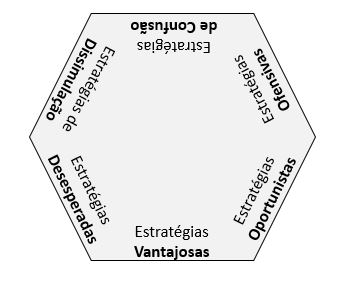
\includegraphics[keepaspectratio]{images/36strategies_intro.jpg}}

}

\caption{Hexágono da 36 estratégias}

\end{figure}%

Cada capítulo deste e-book focará em um dos estratagemas.

Desfrute desta joia escondida!

\part{01 a 06}

\chapter{Estratégias Vantajosas}\label{estratuxe9gias-vantajosas}

Compreendem as estratégias de 01 a 06.

\pandocbounded{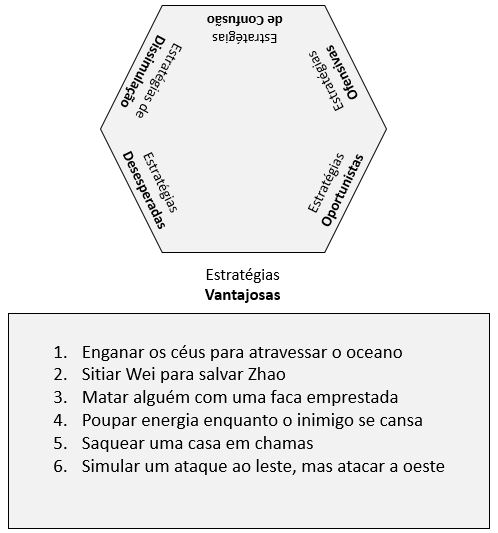
\includegraphics[keepaspectratio]{./images/36strategies_1.jpg}}

\href{estrategia_01.qmd}{1 -- Enganar os céus para atravessar o oceano.}

\href{estrategia_02.qmd}{2 -- Sitiar Wei para salvar Zhao.}

\href{estrategia_03.qmd}{3 -- Matar alguém com uma faca emprestada.}

\href{estrategia_04.qmd}{4 -- Poupar energia enquanto o inimigo se
cansa.}

\href{estrategia_05.qmd}{5 -- Saquear uma casa em chamas.}

\href{estrategia_06.qmd}{6 -- Simular um ataque ao leste, mas atacar a
oeste.}

\chapter{Estratégia 1 - Enganar os céus para atravessar o
oceano}\label{estratuxe9gia-1---enganar-os-cuxe9us-para-atravessar-o-oceano}

Um exército temia atravessar o oceano.

Um conselheiro bolou um plano: combinou uma grande festa com um homem
rico, e o exército inteiro se embebedou na casa deste. Quando esses
acordaram, viram que a casa do homem rico era um barco, e que estavam no
meio do oceano!

A Arte da Guerra diz que ``Toda a guerra é baseada no logro''. Esta
estratégia significa criar algo falso para distrair o inimigo, sob o céu
aberto e atingir o objetivo sem que o mesmo perceba. Se esconder a olhos
vistos!

Essa estratégia funciona porque esperamos que os segredos estejam
escondidos!
\pandocbounded{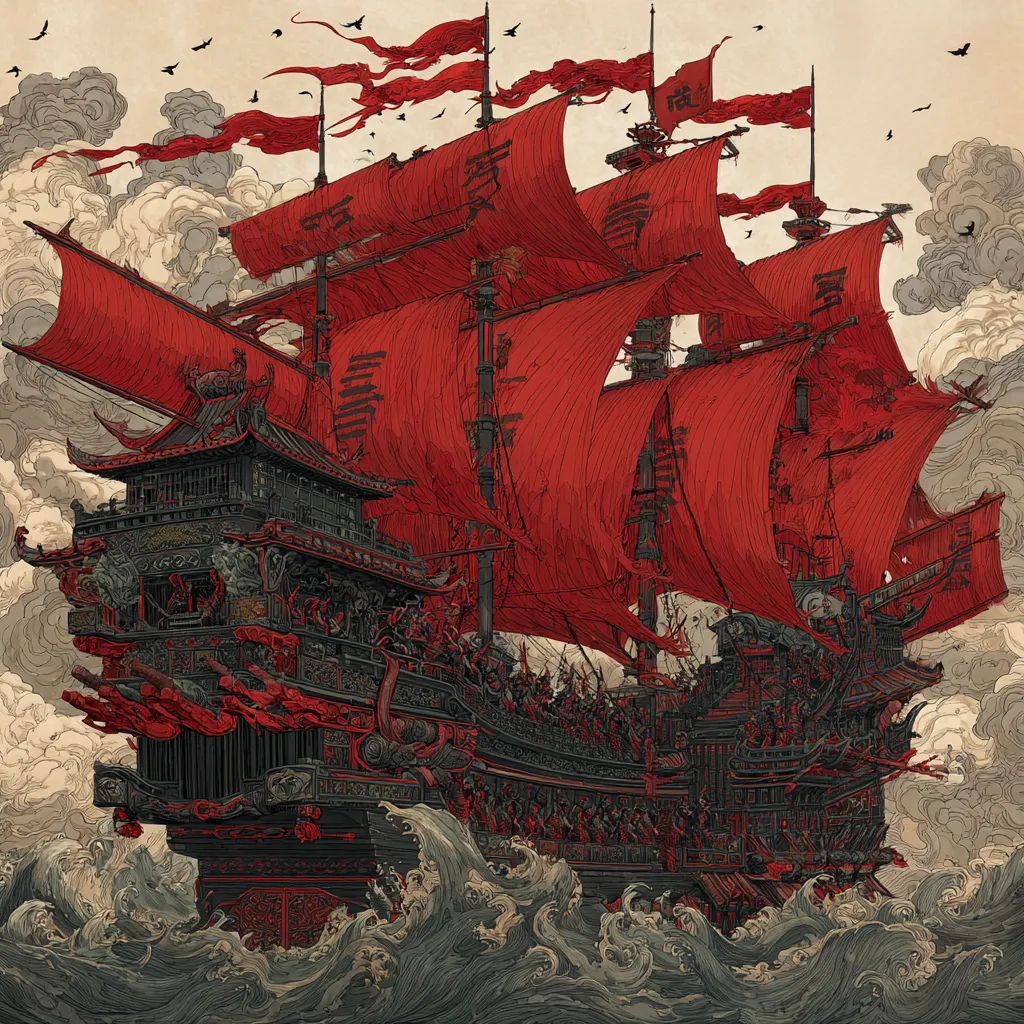
\includegraphics[keepaspectratio]{images/estrategia01.pdf}}

Outro conto que me vem à mente.

O Mulá Nasrudin, todos os dias, cruzava a fronteira montado em seu
burro. Os guardas revistavam a carga, sem nada encontrar de valioso.

\pandocbounded{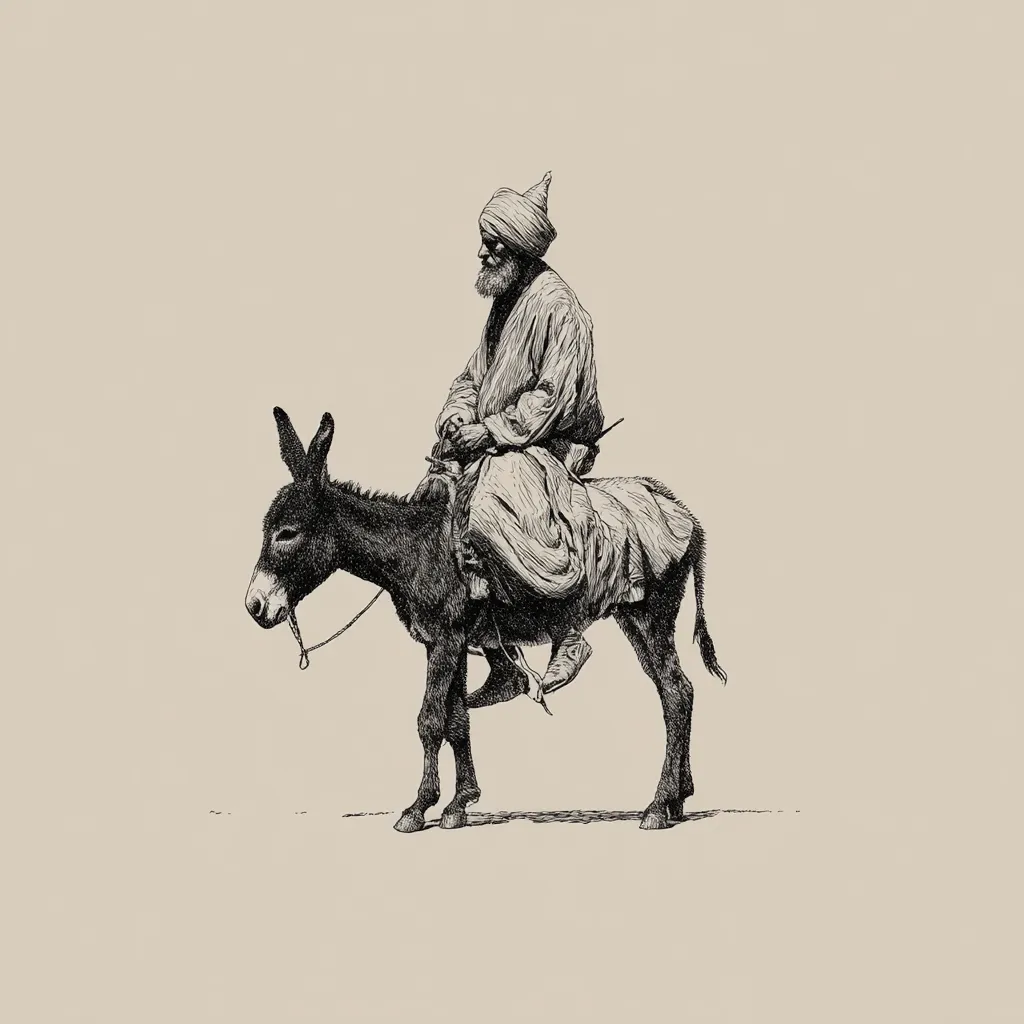
\includegraphics[keepaspectratio]{images/nasrudin_01.png}}

E assim foi, por algumas déc adas, até o dia em que o policial da
fronteira se aposentou e encontrou Nasrudin num bar.

Aí, ele aproveitou e perguntou:

\begin{itemize}
\tightlist
\item
  Mulá, eu sei que você traficava alguma coisa. Como é que você escondia
  a mercadoria? Nunca conseguimos te pegar.
\end{itemize}

Ao que, o Mulá respondeu:

\begin{itemize}
\tightlist
\item
  Ora, eu traficava burros!
\end{itemize}

Esconda a olhos vistos.

``Uma vista familiar não chama a atenção'' - Provérbio chinês

\chapter{Estratégia 2 - Sitiar Wei para salvar
Zhao}\label{estratuxe9gia-2---sitiar-wei-para-salvar-zhao}

O exército de Wei atacou, venceu e sitiou o estado de Zhao.

O exército de Qi, aliado da cidade sitiada, veio em socorro a Zhao. Mas
isto significava batalhar diretamente com o poderoso exército Wei.

\pandocbounded{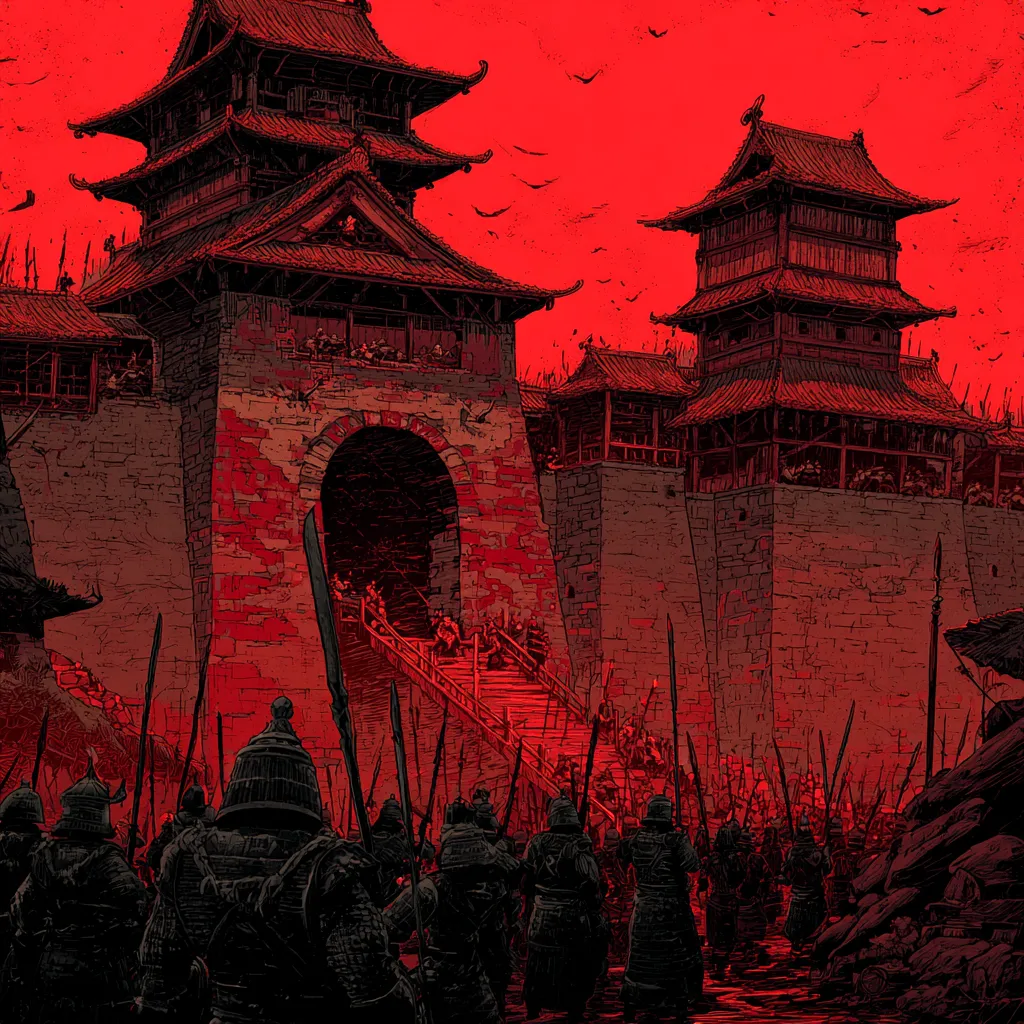
\includegraphics[keepaspectratio]{images/sitiar_wei.png}}

Entretanto, ao invés disso, marcharam em direção à cidade de Wei, que
estava desprotegida de seu exército. Assim que isto ficou claro, o
exército de Wei teve que retornar à sua base, as pressas. Zhao foi
libertada sem batalha alguma! A estratégia significa evitar o ponto
forte do inimigo, e atacar o ponto fraco.

\pandocbounded{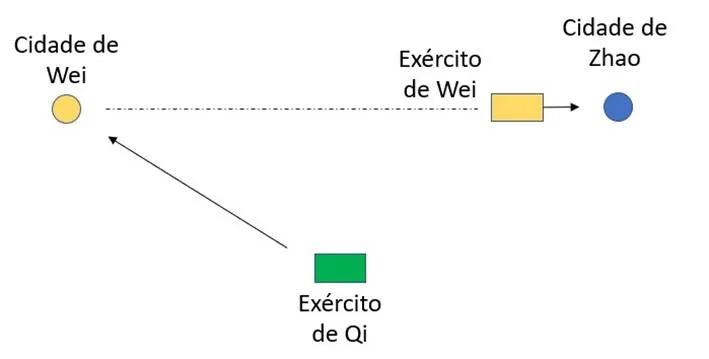
\includegraphics[keepaspectratio]{images/sitiar_wei_2.png}}

O Yin Yang significa sempre ter em mente as forças complementares, a
oposição. Força e Fraqueza, Alto e Baixo.

\pandocbounded{
\includegraphics[keepaspectratio]{images/yin_yang.png}}

Evite o forte, ataque a parte fraca! Evite a parte defendida, ataque na
parte não defendida!

Da mesma forma, a água percorre o caminho do leito do rio e evita as
alturas.

No xadrez, uma forma efetiva de se defender de um ataque é contra-atacar
na ala oposta. Ao ataque na ala do rei, contraataque ao centro ou na ala
da dama!

\chapter{Estratégia 3 - Matar com uma faca
emprestada}\label{estratuxe9gia-3---matar-com-uma-faca-emprestada}

Quando não se tem força suficiente para se opor ao inimigo, utilizar a
força de aliados ou de grupos para tal: é a ``faca emprestada''.

Se você conseguir outros a atuarem em sua causa, você estará utilizando
recursos emprestados para um fim em comum. Uma startup que consegue
acessar recursos, know-how e networking de um grande grupo de
investimentos é um caso desses.

\pandocbounded{
\includegraphics[keepaspectratio]{images/faca.png}}

Este conceito também lembra o de ``cavalo a montar'', de Al Ries e Jack
Trout.

A ideia principal é que, além de ter habilidade, devemos também ter
oportunidades, um cavalo a montar.

\pandocbounded{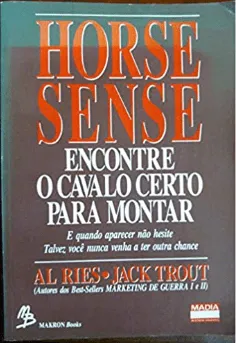
\includegraphics[keepaspectratio]{images/horse.png}}

Por outro lado, o dono do cavalo precisa de bons jóqueis. É uma troca.

O melhor jóquei não é necessariamente o mais leve, esperto ou forte. Ele
também precisa do melhor cavalo. É necessário aliar habilidade com
oportunidades.

De modo genérico, todos nós precisamos estar ligados a um grupo maior, a
aliados, porque é impossível conquistar trabalhar sozinhos. ``Nenhum
homem é uma ilha'', já dizia o autor John Donne.

Esta é a parte 3 das 36 Estratégias de Guerra.

\chapter{Estratégia 4 -- Poupar energia enquanto o inimigo se
cansa}\label{estratuxe9gia-4-poupar-energia-enquanto-o-inimigo-se-cansa}

Saber quando utilizar o tempo e o espaço corretos. Um exemplo é chegar
cedo ao palco da batalha, escolher o melhor lugar -- que tenha a
vantagem natural da altura e do espaço de manobra -- e esperar o inimigo
vir lutando contra o tempo e contra o terreno.

\pandocbounded{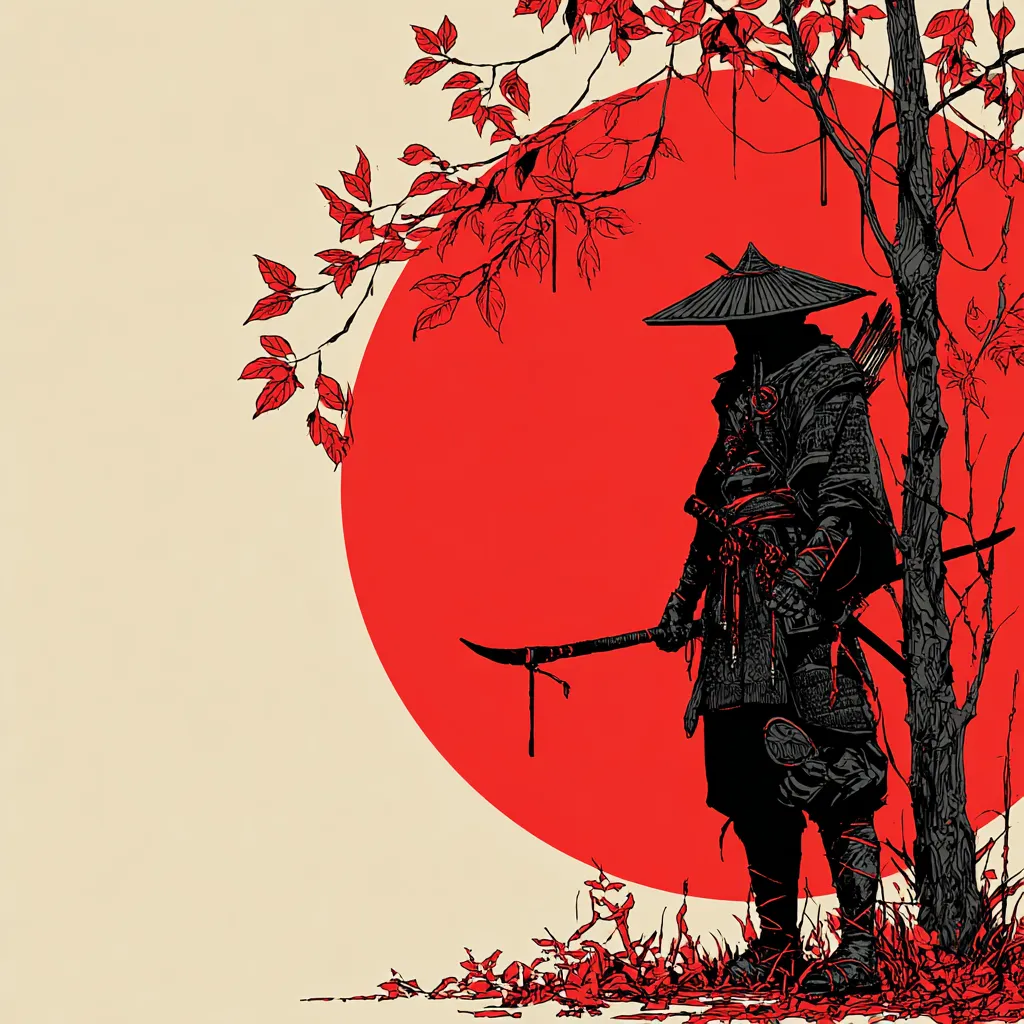
\includegraphics[keepaspectratio]{images/poupar.png}}

``Quem chega primeiro ao campo de batalha e espera o inimigo estará
descansado; quem chega depois e se apressa para lutar estará exausto'' -
Sun Tzu.

Sempre gostei de estudar um pouco todos os dias, e não deixar tudo para
a véspera da prova. Isto é basicamente o oposto do que as pessoas fazem,
que é deixar tudo para a véspera. Dosar energia é fundamental para o
desempenho.

``A energia é como o retesar de uma besta, a decisão, apertar o
gatilho'' - Sun Tzu.

\pandocbounded{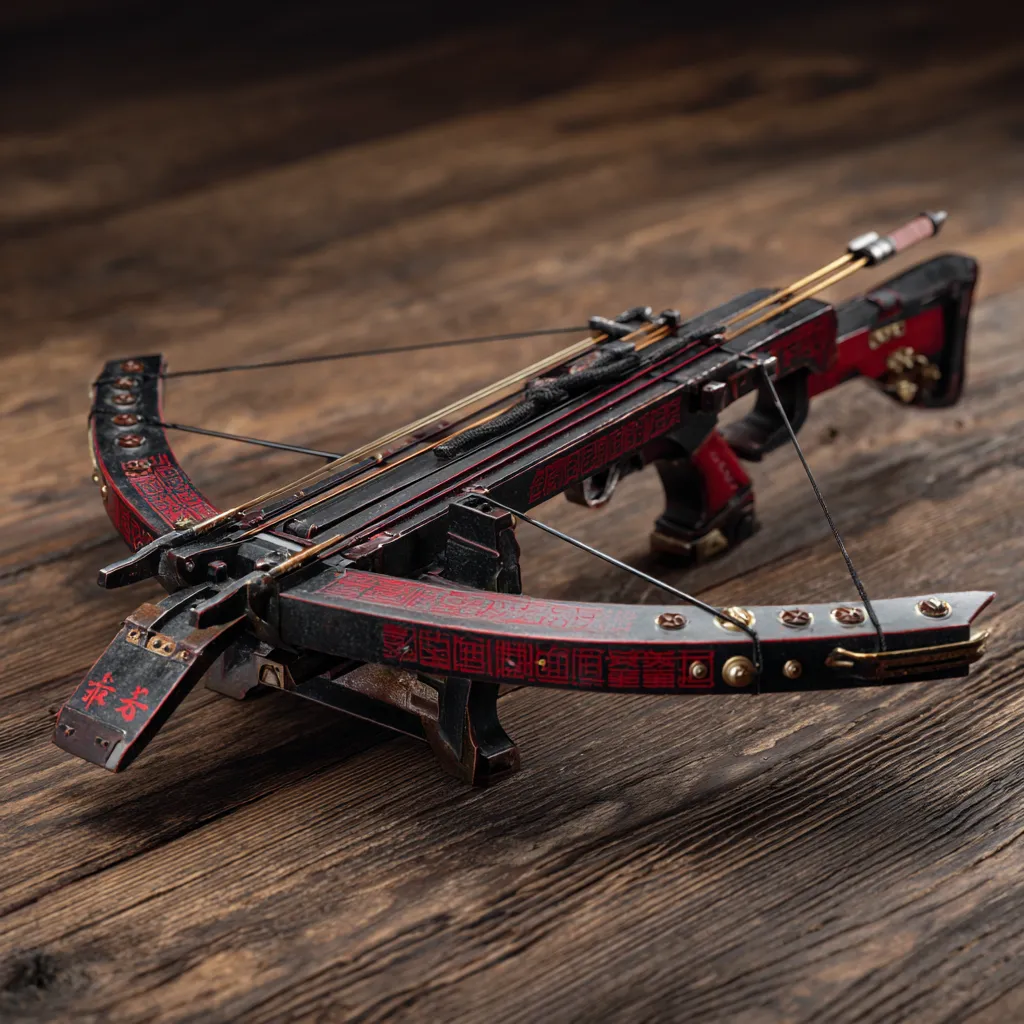
\includegraphics[keepaspectratio]{images/besta.png}}

Também na linha de dosar energia, cada um de nós tem um ciclo diário em
que temos maior concentração. Eu sempre prefiro fazer as tarefas mais
difíceis de manhãzinha, cedinho. Além do mais, estar presente em uma
reunião ou fazer uma tarefa puramente burocrática vai ocupar o seu
tempo, porém não necessariamente vai ser um produto útil para o futuro.
Priorizar fazer o mais difícil e útil no seu pico de energia, e o
burocrático e trabalhoso no seu vale de energia.

Esta é a parte 4 das 36 Estratégias de Guerra.

\chapter{Estratégia 5 - Saquear uma casa em
chamas}\label{estratuxe9gia-5---saquear-uma-casa-em-chamas}

Aproveitar a oportunidade de saquear um lugar quando há caos e confusão.
Quando o inimigo está numa grande crise, este é o momento para atacar.

\pandocbounded{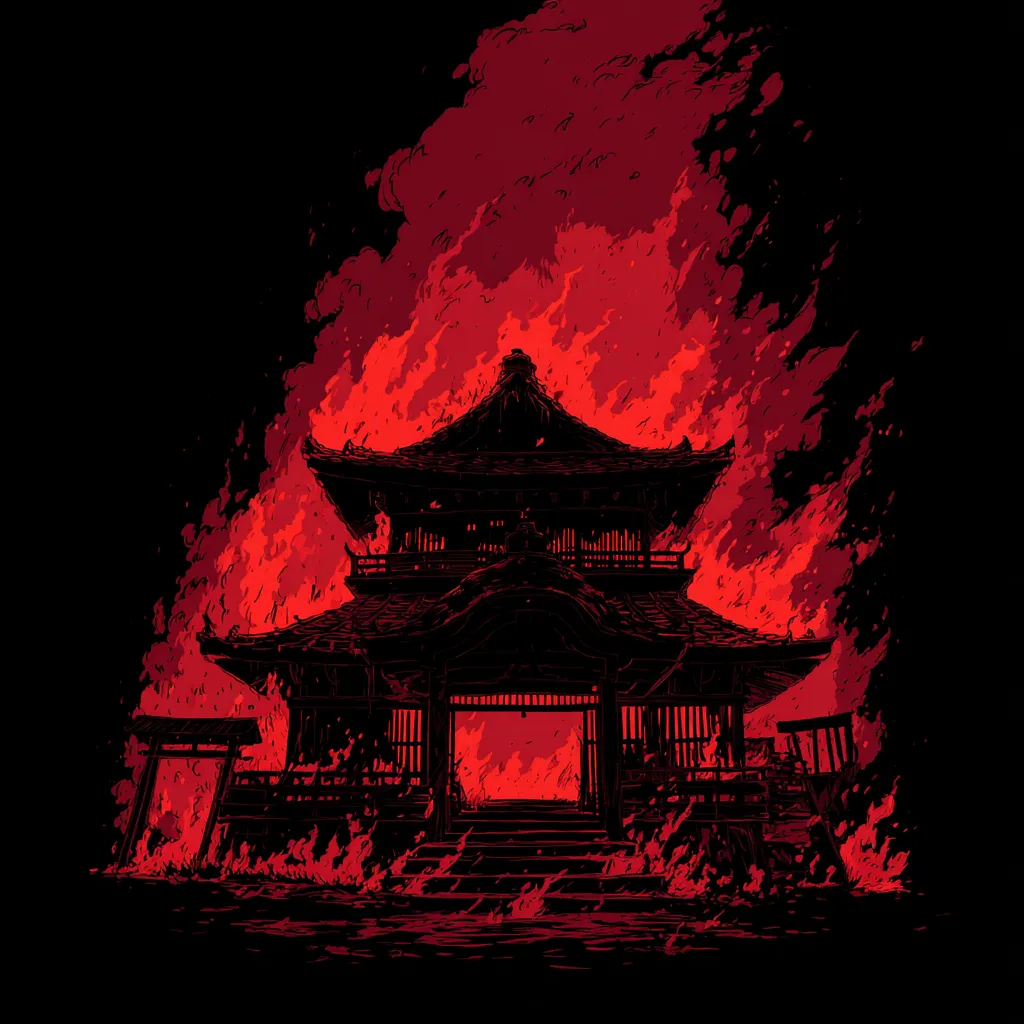
\includegraphics[keepaspectratio]{images/saquear.png}}

Todos temos altos e baixos na vida, e é nos momentos de baixa onde
estamos mais vulneráveis.

Infelizmente, esta é uma técnica bastante utilizada por golpistas. As
pessoas mais propensas a acreditar num ticket de loteria milagroso, ou
num golpe de sorte tipo um jogo do tigrinho, são as mais vulneráveis.

Já dizia Sun Tzu: ``Evite o que é forte e ataque o que é fraco''.

No mundo dos negócios, há empresas e profissionais especializados em
assumir empresas insolventes e prestes a falir, como abutres esperando
pela carniça.

No filme ``O lobo de Wall Street'', o personagem de Leonardo di Caprio
empurra papéis lixo, prometendo retornos enormes, por trás de uma
fachada de boa empresa. Um passo na empresa é empurrar tais papeis para
fundos de pensão, ávidos por grandes retornos (que não virão) e
propensos a acreditarem em aparências.

\pandocbounded{
\includegraphics[keepaspectratio]{images/lobo.png}}

Outro filme ``Uma linda mulher'', o personagem de Richard Gere é um
predador corporativo. Comprar empresas em dificuldade, desmontá-las,
vender partes separadamente e lucrar com isso. Ao longo do filme, há
justamente uma mudança no personagem: ele começa a questionar esse
modelo destrutivo de negócios e considera passar a construir empresas em
vez de apenas desmontá-las.

\pandocbounded{
\includegraphics[keepaspectratio]{images/pretty.png}}

Ação: Tome cuidado, nos inevitáveis momentos de baixa.

Esta é a parte 5 das 36 Estratégias de Guerra.

\chapter{Estratégia 6 -- Simular um ataque ao leste, mas atacar a
oeste}\label{estratuxe9gia-6-simular-um-ataque-ao-leste-mas-atacar-a-oeste}

A dissimulação está na essência da estratégia. O inimigo não pode
concentrar forças em todos os lugares. A estratégia consiste em ocultar
as suas verdadeiras intenções e fazer o inimigo concentrar forças no
local errado.

\pandocbounded{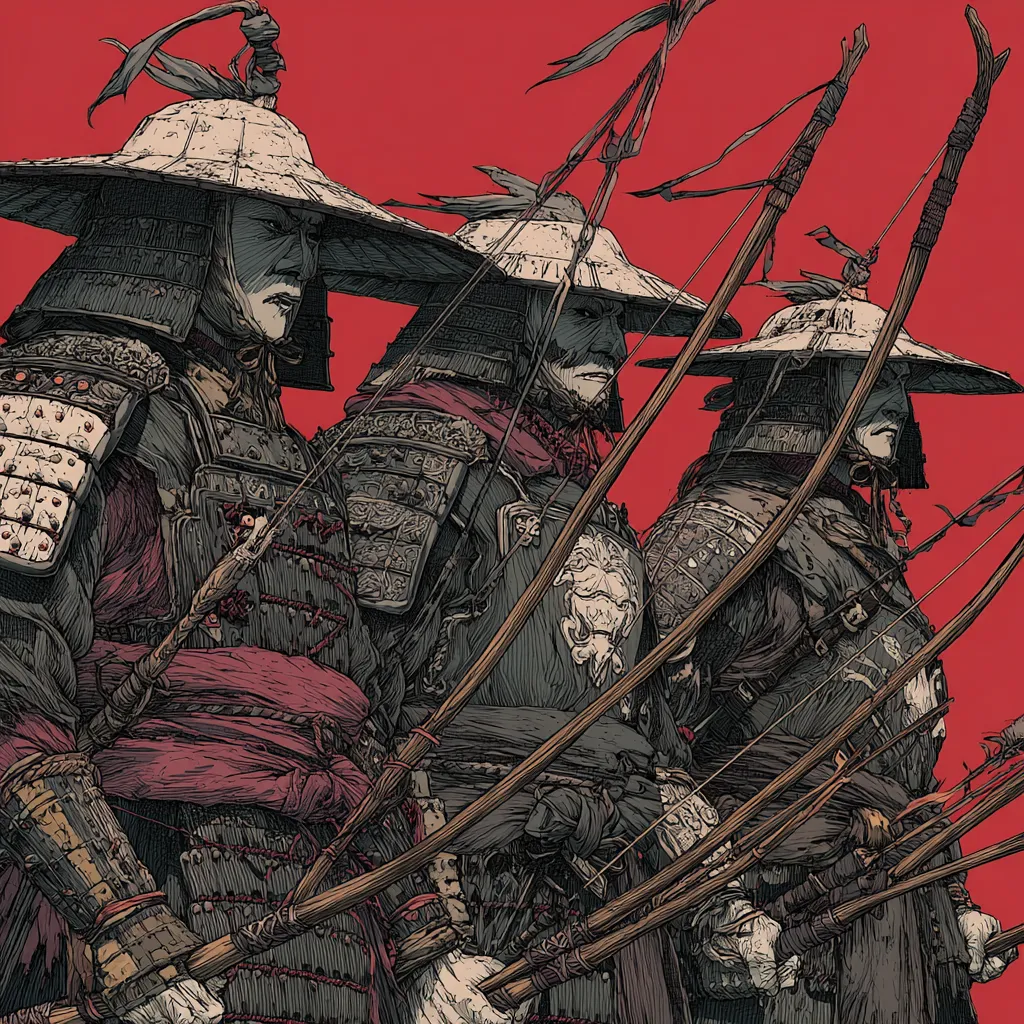
\includegraphics[keepaspectratio]{images/simular.png}}

Já dizia Sun Tzu: ``Se você se defende a leste, estará vulnerável a
oeste. Se você se defende a oeste, estará vulnerável a leste. Se você se
defender em todos os pontos, estará vulnerável em todos os pontos''.

Portanto, devemos acertar qual o foco para conseguirmos ser efetivos.

E, também de Sun Tzu: ``Toda a guerra é baseada em enganar o oponente''.

Um jogador de futebol que aparenta um drible para a direita, mas vai
para a esquerda. Um jogador de poker que blefa com as cartas que tem.

\pandocbounded{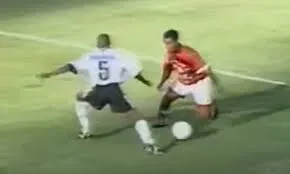
\includegraphics[keepaspectratio]{images/romario.png}}
Para qual lado vai o Romário?

No Dia-D, invasão da Europa pelas forças aliadas, a dissimulação foi tão
bem sucedida que, mesmo após a invasão ter sido realizada, o alto
comando nazista não acreditava que isto estivesse ocorrendo.

Não seja tão transparente em suas intenções, quando tiver um oponente.
Dê um drible nele.

Esta é a parte 6 das 36 Estratégias de Guerra.

\part{07 a 12}

\chapter{Estratégias Oportunistas}\label{estratuxe9gias-oportunistas}

Compreendem as estratégias de 07 a 12.

\pandocbounded{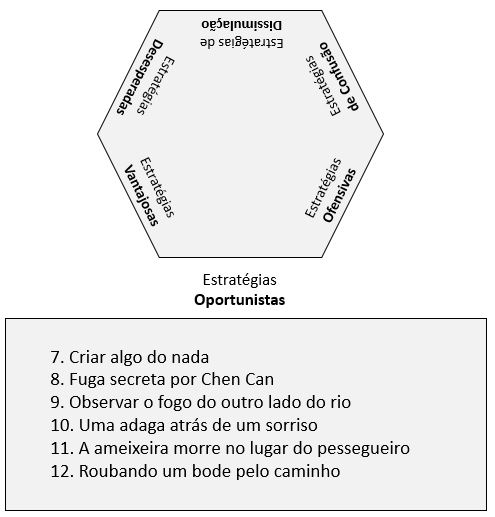
\includegraphics[keepaspectratio]{images/36strategies_2.jpg}}

\href{estrategia_07.qmd}{7 -- Criar algo do nada.}

\href{estrategia_08.qmd}{8 -- Fuga secreta por Chen Can.}

\href{estrategia_09.qmd}{9 -- Observar o fogo do outro lado do rio.}

\href{estrategia_10.qmd}{10 -- Uma adaga atrás de um sorriso.}

\href{estrategia_11.qmd}{11 -- A ameixeira morre no lugar do
pessegueiro.}

\href{estrategia_12.qmd}{12 -- Roubando um bode pelo caminho.}

\chapter{Estratégia 7 - Criar algo do
nada}\label{estratuxe9gia-7---criar-algo-do-nada}

``Nada se perde, nada se cria, tudo se transforma'', já dizia Lavoisier.
Se é assim, como podemos criar algo do nada?

Obviamente, não criamos matéria do nada no sentido físico, mas podemos
algo de valor para o ser humano a partir de coisas com pouco valor.

\pandocbounded{
\includegraphics[keepaspectratio]{images/nada.png}}

Uma empresa, uma startup, consiste em criar um empreendimento do zero e
fazê-lo prosperar.

A agricultura não é nada menos que entender, usar e cuidar de recursos
da natureza para que consigamos colher os frutos.

Uma sucessão de blefes pode dar certo, se os atores envolvidos
acreditarem neste. Um ditado popular no Vale do Silício é o ``Fake it
until you make it'', imite o que você quer ser até conseguir.

Ninguém nasce pronto para a posição que quer ocupar. Todos são, em algum
momento e em alguma medida, iniciantes, apenas pedras brutas em
potencial que devem ser lapidadas com o tempo.

Um bom exemplo é a história (fictícia) do genro do Bill Gates:

Pai: -- Filho, escolhi uma ótima moça para você casar. Filho: -- Mas
pai, eu prefiro escolher a minha mulher. Pai: -- Ela é filha do Bill
Gates\ldots{} Filho: -- Bem, neste caso, eu aceito.

Então, o pai vai encontrar o Bill Gates. Pai: -- Bill, eu tenho o marido
para a sua filha! Bill Gates: -- Mas a minha filha é muito jovem para
casar! Pai: -- Mas este jovem é vice-presidente do Banco Mundial\ldots{}
Bill Gates: -- Neste caso, tudo bem.

Finalmente, o pai vai ao Presidente do Banco Mundial. Pai: -- Senhor
Presidente, eu tenho um jovem muito bem recomendado para ser
vice-presidente do Banco Mundial. Pres.~Banco Mundial: -- Mas eu já
tenho muitos vice-presidentes. Pai: -- Mas senhor, este jovem é genro do
Bill Gates. Pres.~Banco Mundial: -- Neste caso ele pode começar amanhã
mesmo!

\section{Criar uma linhagem nobre do
nada}\label{criar-uma-linhagem-nobre-do-nada}

O grande unificador do Japão, Toyotomi Hideyoshi, já tinha conquistado
militarmente todo o território. Porém, no Japão, a autoridade do
Imperador era muito respeitada como uma figura divina -- pense no
Imperador como um Papa, ao invés da noção usual de grande conquistador.

Para legitimar a sua autoridade, Hideyoshi precisava de um cargo
equivalente a Primeiro-Ministro, ou regente, do Japão. Porém, sendo de
origem camponesa, ele não tinha uma linhagem nobre para assumir o papel.

Assim, ele passou a cortejar a nobre família Fujiwara, oferendo mimos e
paparicos. Depois de um tempo, surpreendentemente ``descobriram'' uma
relação de antepassados antiga entre Hideyoshi e os Fujiwara. Com isso,
Hideyoshi conseguiu ser nomeado regente do Imperador, legitimando a
posição de domínio sobre todo o Japão.

\section{Sopa de pedra}\label{sopa-de-pedra}

Outro exemplo é a história da sopa de pedra.

\pandocbounded{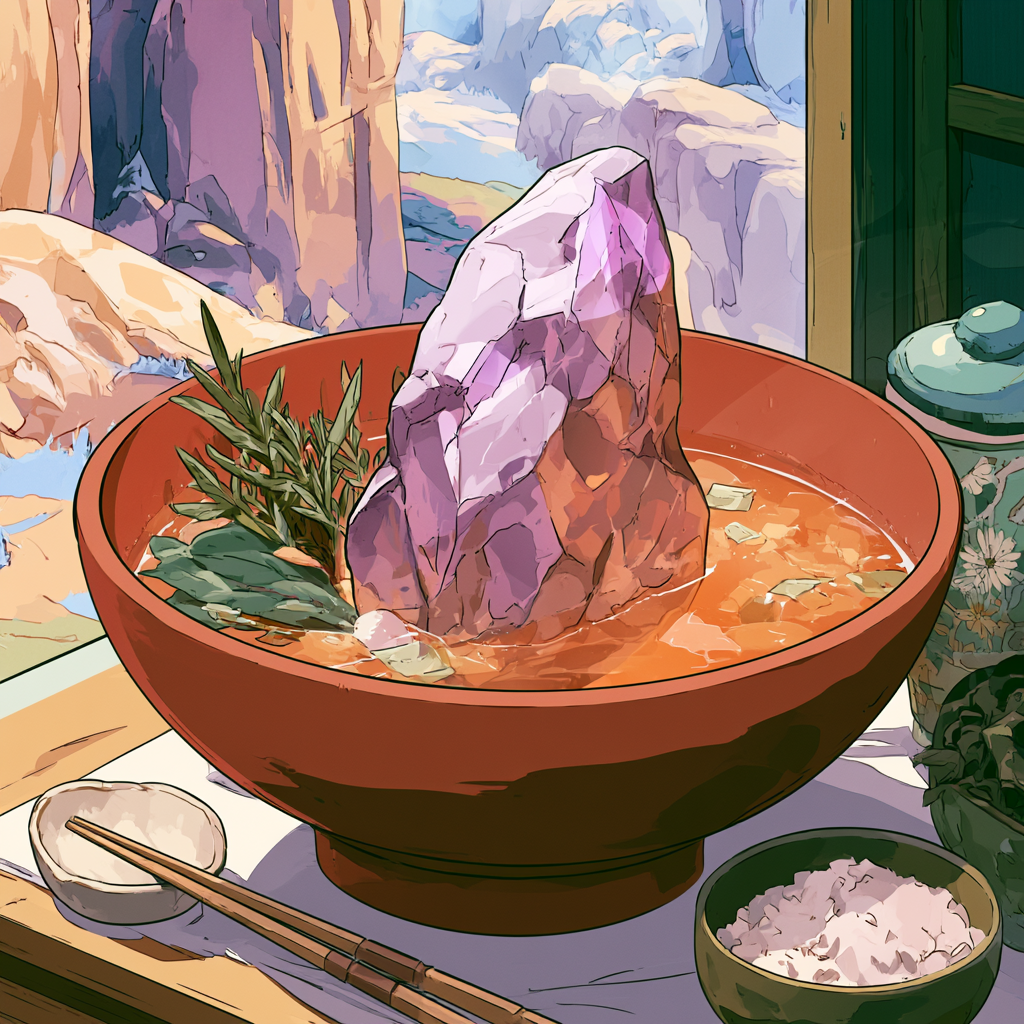
\includegraphics[keepaspectratio]{images/sopa_pedra.png}}

Um viajante, sem nada, chega numa cidade e fala que vai fazer sopa de
pedra. Os habitantes, intrigados, lhe fornecem água, panelas e fogo. O
viajante começa a cozinhar uma pedra, sem pressa, sob os olhares
curiosos. Com o fervor da água, ele começa a pedir alguns ingredientes
básicos: cenoura, sal. Depois, outros ingredientes mais elaborados:
macarrão, carne, até que consegue uma excelente ``sopa de pedra''.

Esta é a parte 7 das 36 Estratégias de Guerra.

\chapter{Estratégia 8 -- Fuga secreta por Chen
Can}\label{estratuxe9gia-8-fuga-secreta-por-chen-can}

Atingir o inimigo pela retaguarda, onde ele estiver desprotegido, e de
forma inesperada.

Esta estratégia deriva de uma história de Lui Bang, 200 a.C., que viria
posteriormente a ser imperador da China. O exército de Liu Bang estava
em retirada, e mandou destruir todas as pontes que acessavam o seu
acampamento. Meses depois, ele ordenou que reconstruíssem as pontes.

O inimigo, desconfiado, passou a se preparar para um ataque iminente
pela pontes. Mas, para surpresa do inimigo, Liu Bang utilizou a passagem
secreta de Chen Can, contornando as montanhas por um longo caminho, para
um ataque-surpresa.

\pandocbounded{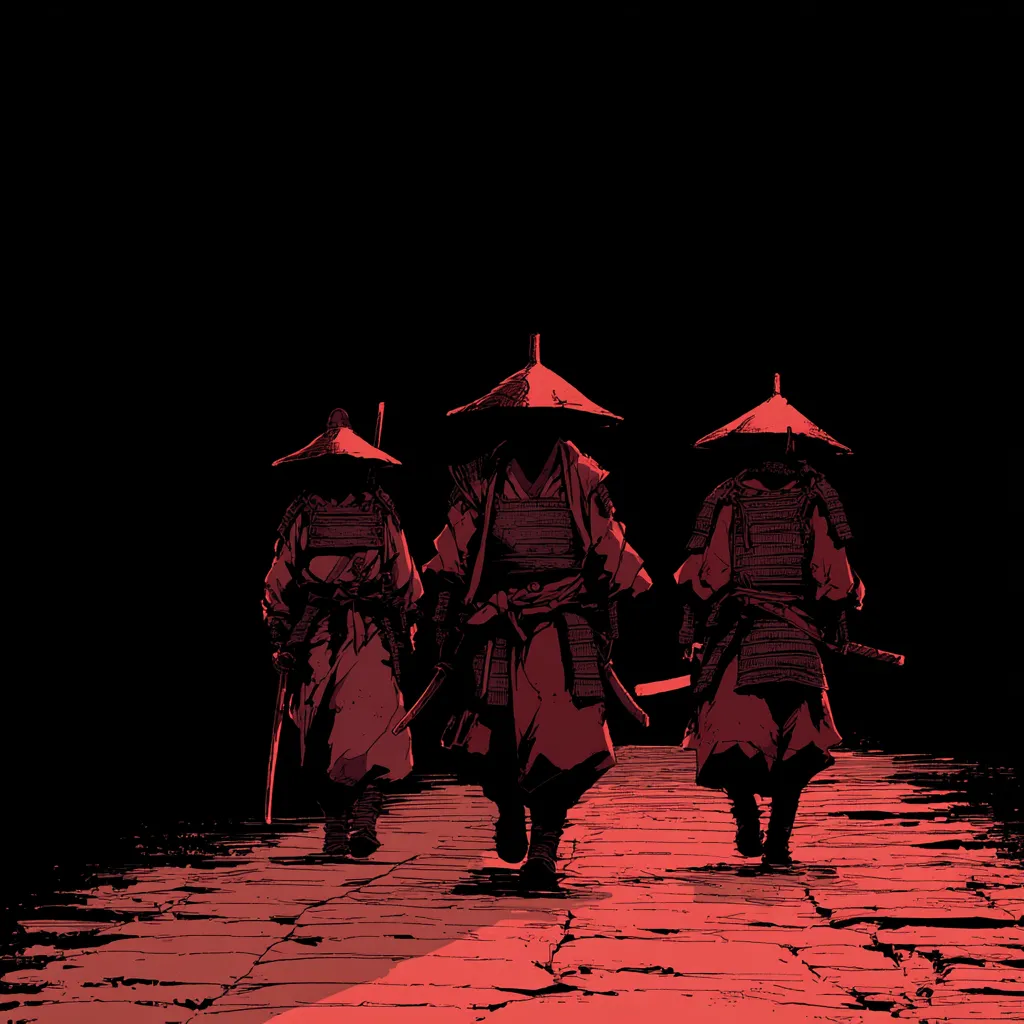
\includegraphics[keepaspectratio]{images/fuga.png}}

É uma estratégia de surpreender o oponente, através de algum atalho
desconhecido por ele.

No Xadrez, isto é bem comum. Um gambito cheio de armadilhas vai pegar o
amador desconhecido.

Em termos de um trabalho técnico, ter conhecimento adicional sobre como
o processo funciona de verdade, ou quem é a pessoa correta a contatar
para desenrolar um assunto, ou alguma técnica apurada de algoritmos é o
equivalente a um atalho para chegar ao objetivo final.

\chapter{Estratégia 9 - Observar o fogo do outro lado do
rio}\label{estratuxe9gia-9---observar-o-fogo-do-outro-lado-do-rio}

Quando houver desordem e lutas internas entre as forças do inimigo,
deve-se esperar enquanto este se enfraquece.

Ou, como disse Napoleão Bonaparte, ``Nunca interrompa o inimigo quando
ele estiver cometendo um erro''

\pandocbounded{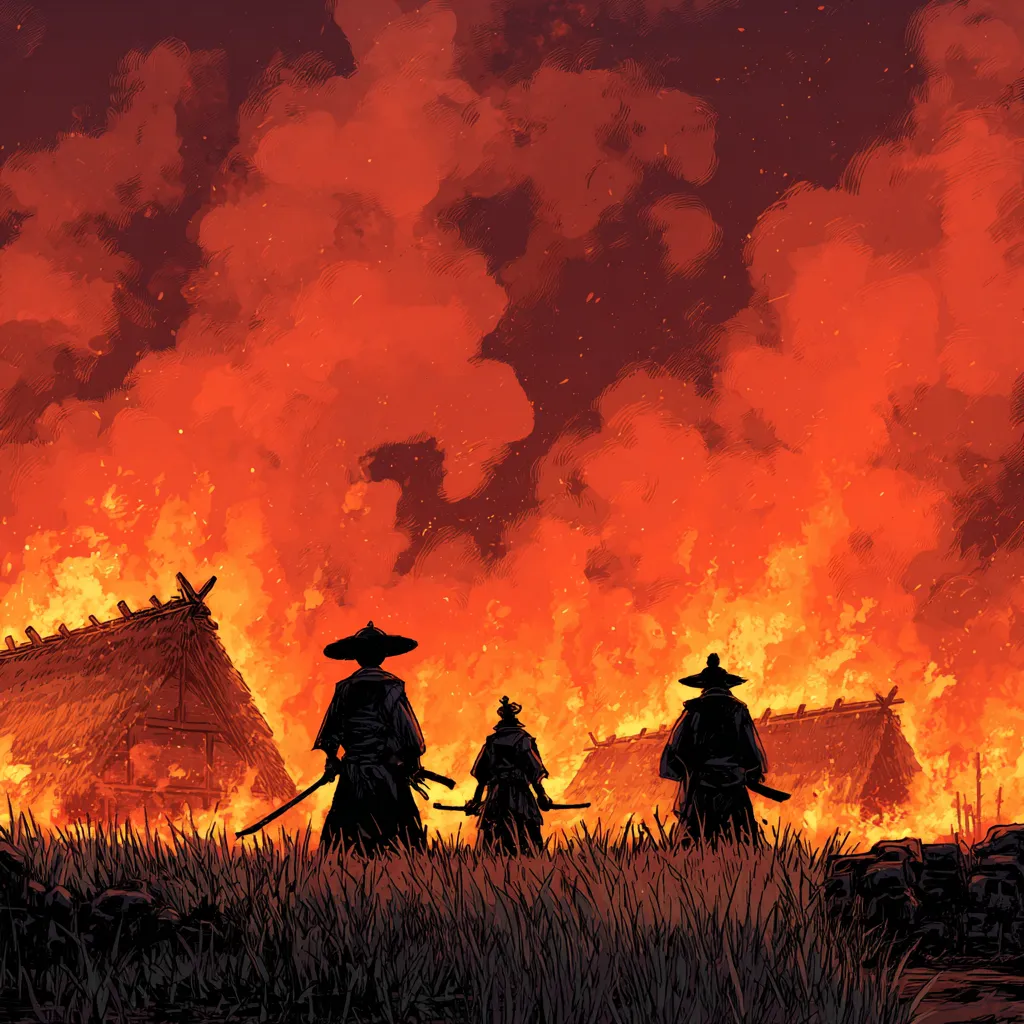
\includegraphics[keepaspectratio]{images/fogo.png}}

Isso também lembra um conto de Esopo. Estavam um leão e um urso brigando
por um pedaço de carne.

\pandocbounded{
\includegraphics[keepaspectratio]{images/leao_urso.png}}

O primeiro, por se achar no direito de ter uma porcentagem, dado ser o
rei da selva. O segundo, por ter feito a caça. Uma raposa ficou
escondida, vendo tudo, e esperou eles se digladiarem por algum tempo.
Até, que, subitamente, a raposa pegou a carne e fugiu correndo\ldots{}

Esta é a parte 9 das 36 Estratégias de Guerra.

\chapter{Estratégia 10 - Uma adaga atrás de um
sorriso}\label{estratuxe9gia-10---uma-adaga-atruxe1s-de-um-sorriso}

Conquistar a confiança do inimigo, para desarmá-lo. O que parece fraco
(macio) por fora, pode ser forte (duro) por dentro. Esconda uma adaga
atrás de um sorriso.

\pandocbounded{
\includegraphics[keepaspectratio]{images/adaga.png}}

Na Arte da Guerra de Sun Tzu, há uma frase memorável a respeito:

Quando capaz, finja incapacidade; quando ativo, finja inativo. Quando
perto do objetivo, finja estar muito longe; quando muito longe, faça com
que pareça perto.

Por outro lado, não confie em sorrisos, palavras amigáveis.

Algumas das piores pessoas que conheci eram muito agradáveis por fora.

Confie nos atos da pessoa, no que ela faz, não no que ela diz. No mundo
financeiro, o autor Nassim Taleb diz, de forma equivalente, ``mostre-me
sua carteira de investimentos'', mostre o que você faz, e não apenas
palavras.

Esta é a parte 10 das 36 Estratégias de Guerra.

\chapter{Estratégia 11 -- A ameixeira morre no lugar do
pessegueiro}\label{estratuxe9gia-11-a-ameixeira-morre-no-lugar-do-pessegueiro}

Fazer sacrifícios quando perdas são inevitáveis. O poema significa que
essas duas árvores são tão íntimas que uma está disposta a morrer pela
outra.

É o popular ``perder os anéis para salvar os dedos''. Perder uma batalha
para salvar a guerra. Perder um cavalo para salvar a dama.

\pandocbounded{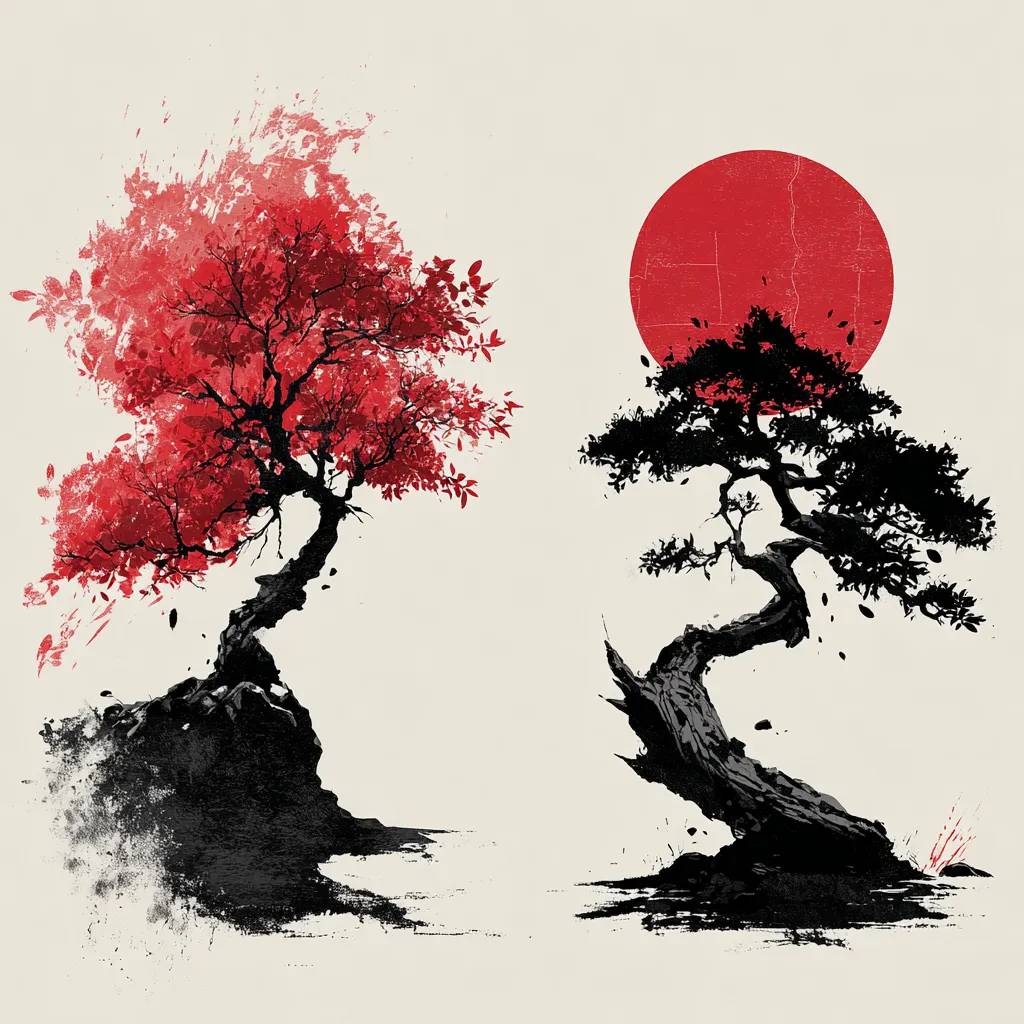
\includegraphics[keepaspectratio]{images/ameixeira.png}}

Uma empresa, quando em crescimento e com capital sobrando, usa o mesmo
para expandir sua linha de produtos e comprar outras empresas. Quando a
maré muda, é o oposto: é preferível sacrificar linhas de produto e
fechar fábricas do que tentar manter tudo e perder tudo.

Exemplo: A corrida entre Tian Ji e Sun Bin

Tian Ji e Sun Bin, dois generais da antiguidade, tinham 3 cavalos cada,
e eles eram equivalentes: tanto o mais rápido, o médio e o mais fraco
chegavam praticamente empatados.

Sun Bin pensou numa forma de vencer a disputa, sacrificando um de seus
cavalos: fez o seu mais lento correr e perder contra o mais rápido do
oponente. A seguir, o seu cavalo médio venceu o cavalo mais lento, e o
seu mais rápido venceu o médio do oponente.

\pandocbounded{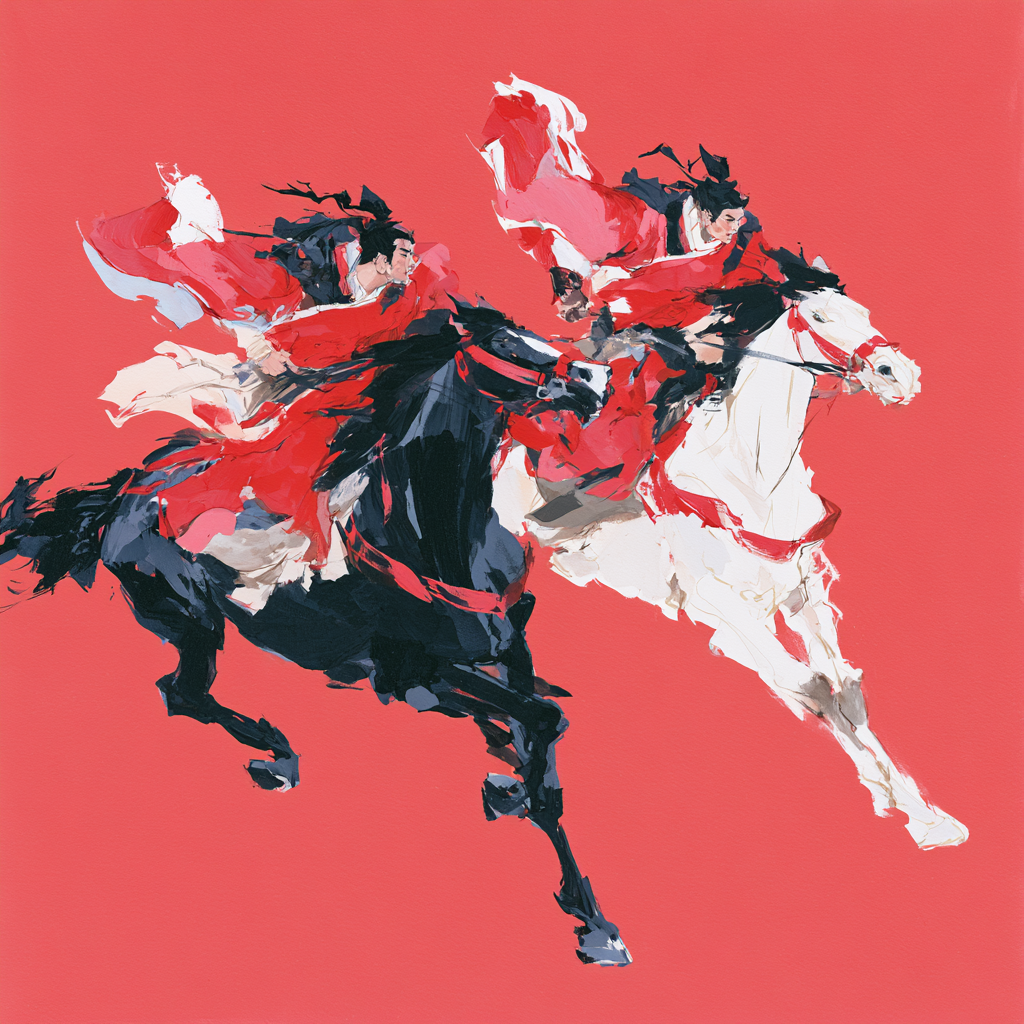
\includegraphics[keepaspectratio]{./images/two_horses_running_a_race.png}}

Em ocasião de batalha, Sun Bin fez o mesmo: sacrificava a parte fraca de
seu exército para distrair a atenção da parte forte do inimigo, para
então utilizar o seu ponto forte contra a parte fraca do oponente,
causando estrago extremamente maior.

Em nível pessoal. Sempre queremos fazer mais coisas do que somos
capazes. Digamos, eu quero fazer aulas de violino, porém, não tenho
tempo livre e estou priorizando estudar uma nova ferramenta
computacional. Desejos são infinitos, nosso tempo e capacidade
cognitiva, não. Necessariamente temos que priorizar, de alguma forma.
Ter tempo é uma questão de priorização.

É a lei do sacríficio, uma das 22 leis do marketing de Al Ries e Jack
Trout: ``para conseguir uma coisa, você deve sacrificar todas as
outras''.

Segundo o economista Grigory Mankiw, uma das leis da Economia é o
\textbf{custo de oportunidade}. O verdadeiro custo de você optar por
algo é desistir de todas as outras opções. O custo de oportunidade está
presente em todas as facetas de nossas vidas.

``A vida é como um self service. Você pode pegar o que quiser, mas tem
que pagar por isso'' - Gilcler Regina

Esta é a parte 11 das 36 Estratégias de Guerra.

\chapter{Estratégia 12 -- Roubando um bode pelo
caminho}\label{estratuxe9gia-12-roubando-um-bode-pelo-caminho}

Aproveitar uma oportunidade de ganho fácil, por menor que seja.
Aproveitar as vantagens que surgem pelo caminho. Aproveitar os erros do
seu adversário.

\pandocbounded{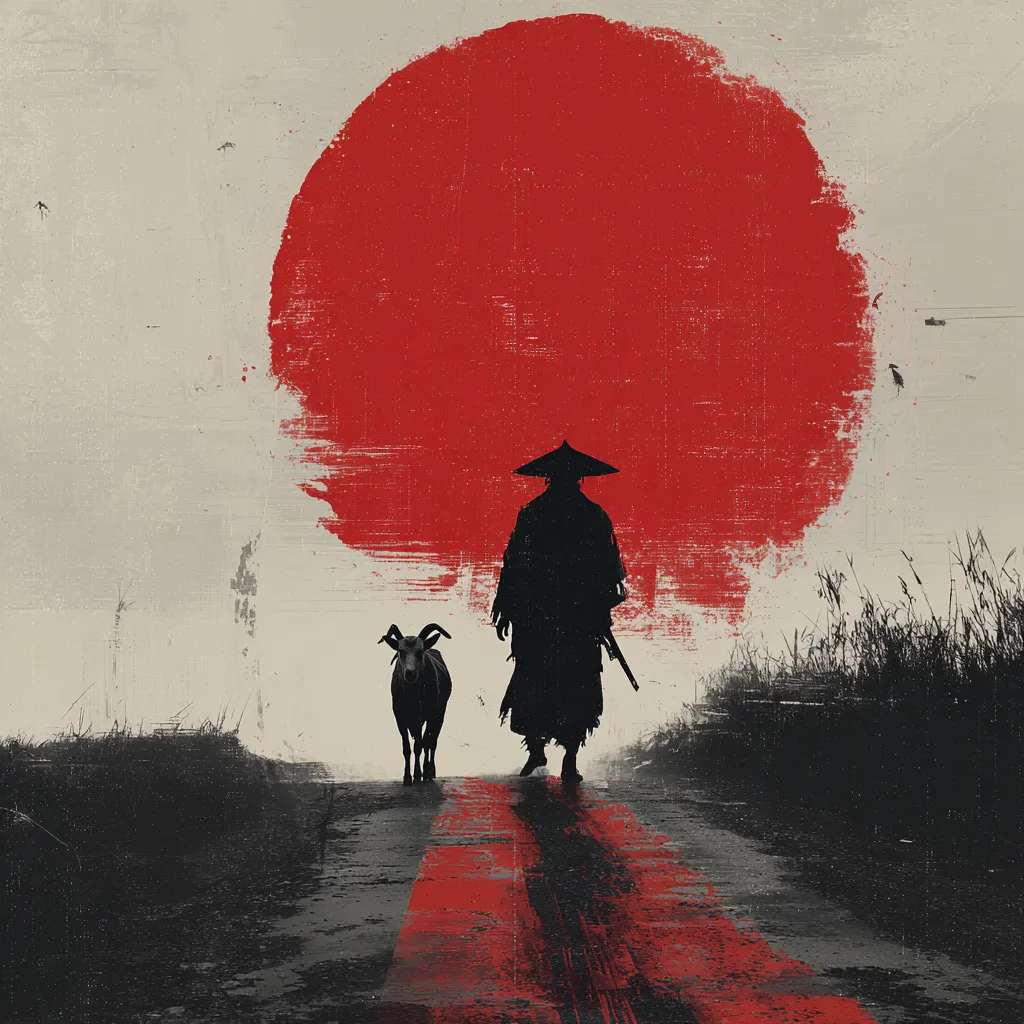
\includegraphics[keepaspectratio]{images/bode.png}}

Quando eu trabalhava na Aeronáutica, surgiu a oportunidade de fazer um
MBA em Gerência de Projetos. É que é assim, a área estima uma quantidade
de vagas, pede todos os anos, e muito de vez em quando alguns desses
pedidos eram contemplados.

Pois bem, neste ano em específico, tinham duas vagas, e nenhum dos
oficiais mais antigos do que eu queria fazer, por diversos motivos (já
estavam fazendo outras atividades, tinham outro trabalho paralelo, etc).

Eu também tinha um problema: já estava fazendo mestrado em Eletrônica na
UFRJ\ldots{} e trabalhando na Aeronáutica. Aceitei assim mesmo, se
tivesse que me matar por dois anos para concluir tudo, que assim fosse.
Eu era solteiro e jovem, então o timing era bom para isso.

Um MBA a mais no currículo não é nada mau.

\pandocbounded{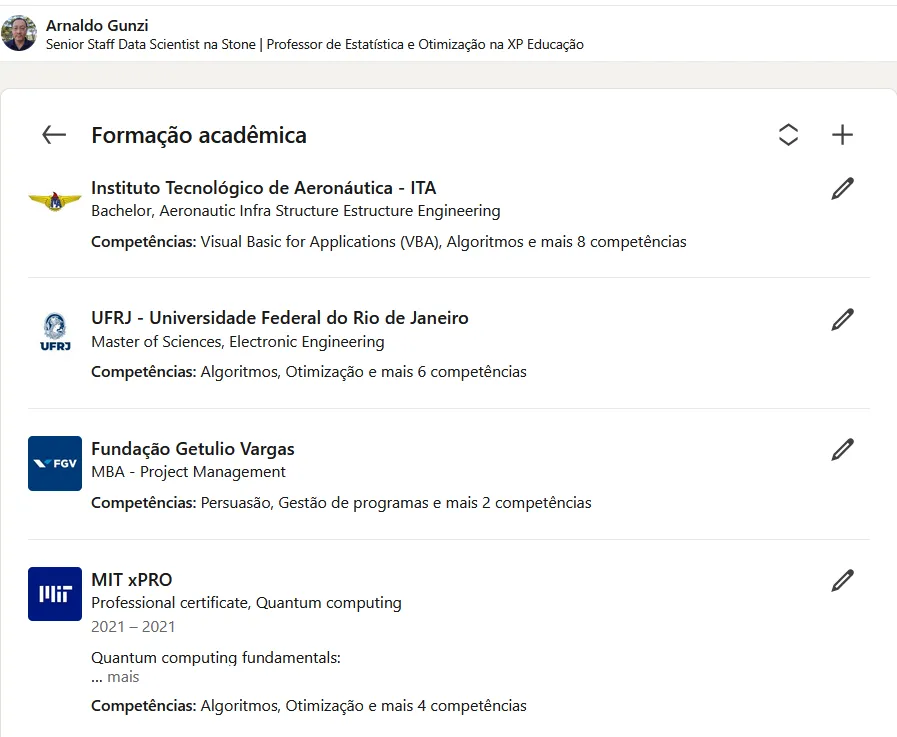
\includegraphics[keepaspectratio]{images/mba.png}}

Bom, em resumo, ``roubei o bode'' que surgiu no meu caminho.

No xadrez, quando jogam dois grandes mestres de alto nível, o jogo tende
a empatar, então eles devem aproveitar qualquer imprecisão mínima na
jogada do outro.

Muita gente recusa oportunidades por ``não estarem preparados'', estarem
``ocupados'' ou coisa similar.

Já dizia Pasteur, ``A sorte favorece a mente preparada''.

Olha, não é todo dia que surge um bode de graça no caminho. Nas raras
ocasiões em que isso acontecer, aproveite! Nunca mais a oportunidade
aparecerá novamente.

Esta é a parte 12 das 36 Estratégias de Guerra.

\part{13 a 18}

\chapter{Estratégias Ofensivas}\label{estratuxe9gias-ofensivas}

Compreendem as estratégias de 13 a 18.

\pandocbounded{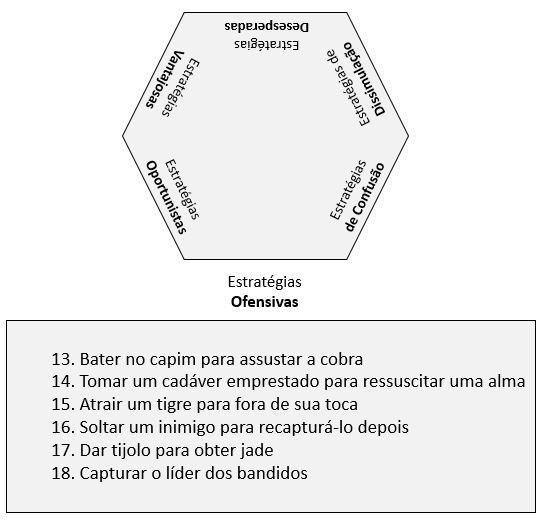
\includegraphics[keepaspectratio]{./images/36strategies_3.jpg}}

\href{estrategia_13.qmd}{13 -- Bater no capim para assustar a cobra.}

\href{estrategia_14.qmd}{14 -- Tomar um cadáver emprestado para
ressuscitar uma alma.}

\href{estrategia_15.qmd}{15 -- Atrair um tigre para fora de sua toca.}

\href{estrategia_16.qmd}{16 -- Soltar um inimigo para recapturá-lo
depois.}

\href{estrategia_17.qmd}{17 -- Dar tijolo para obter jade.}

\href{estrategia_18.qmd}{18 -- Capturar o líder dos bandidos.}

\chapter{Estratégia 13 - Bater no capim para assustar a
cobra}\label{estratuxe9gia-13---bater-no-capim-para-assustar-a-cobra}

Ao invés de capturar a cobra, deve-se assustá-la dando batidas no capim,
e fazer a captura quando ela aparecer. É uma estratégia ofensiva, para
fazer o inimigo revelar as cartas que tem na manga.

É como uma reunião inicial, para tentar dar uma sondada nas intenções do
interlocutor.

\pandocbounded{
\includegraphics[keepaspectratio]{./images/snake_in_the_grass.png}}

Um exemplo é fazer um lance inicial alto num leilão, para testar quem
quer realmente bancar a concorrência.

No contexto de uma empresa, é comum fazermos testes piloto de uma
alteração no processo, ou utilizar um novo fornecedor aos poucos. Ou,
utilizando terminologia de inovação, fazer um produto mínimo viável
(MVP).

Se o novo processo rodar bem, o fornecedor for bom ou a recepção do
público for boa, podemos pegar o teste inicial e produtizar o mesmo de
forma mais robusta.

Num contexto mais romântico, um primeiro encontro ou um início de namoro
vai te dar infinitamente mais informação do que podemos obter sobre a
pessoa na internet.

Quem sabe, você não evita uma verdadeira cobra!

\chapter{Estratégia 14 - Tomar um cadáver emprestado para ressuscitar
uma
alma}\label{estratuxe9gia-14---tomar-um-caduxe1ver-emprestado-para-ressuscitar-uma-alma}

Uma pessoa fraca pode requerer sua assistência para ficar forte e
conseguir se opor ao inimigo. Por outro lado, mesmo o exército forte
precisa da ajuda de vários exércitos fracos para chegar aos seus
objetivos.

\pandocbounded{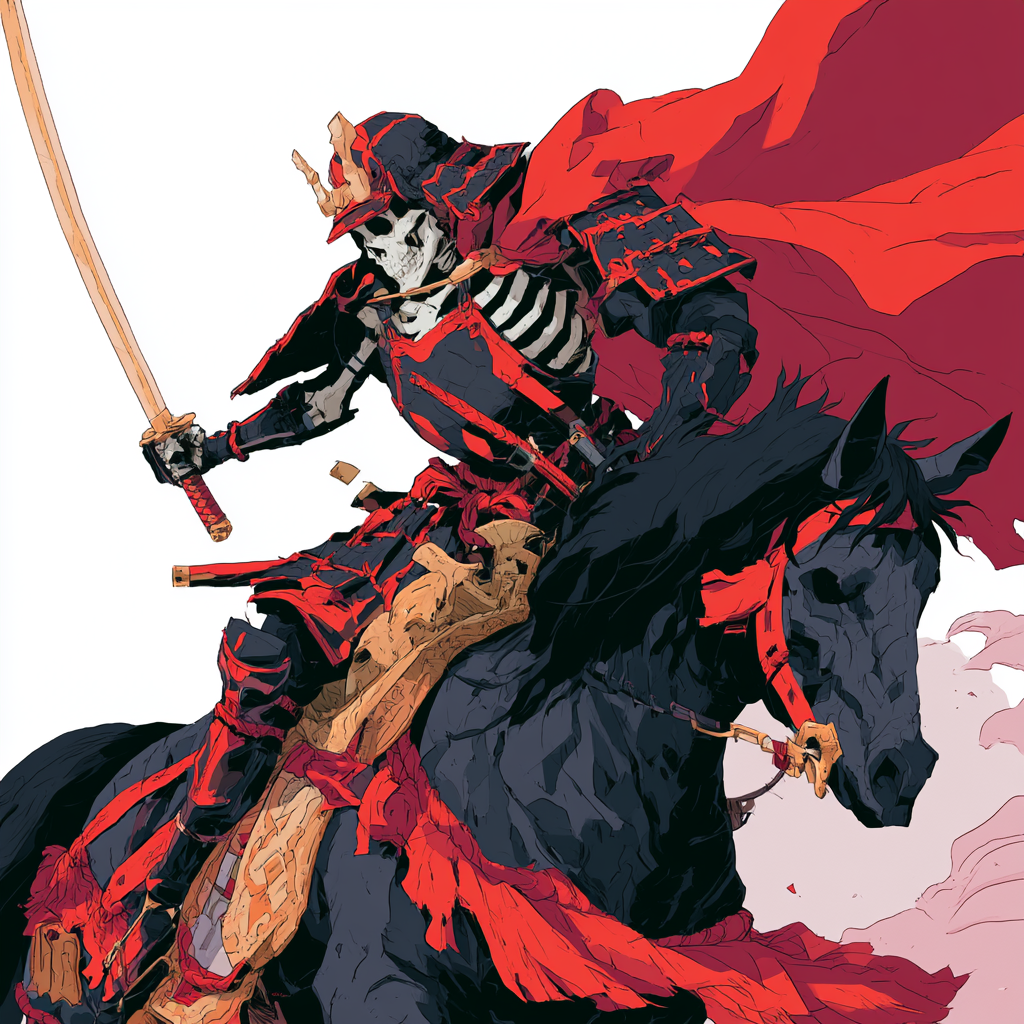
\includegraphics[keepaspectratio]{./images/skeleton_in_a_warrior_armor.png}}

Um exemplo muito bom é o Natal. Jesus não nasceu no dia 25 de dezembro.
O Natal no dia 25/dez só surgiu no século IV, aproveitando que vários
povos já comemoravam esta data como sendo o solstício de inverno. Ou
seja, tomaram um cadáver (data comemorativa de povos conquistados pelo
Império Romano) para ressuscitar uma alma (tomar para si esta
comemoração).

Há inúmeros outros exemplos na história. Imperadores fantoche ocorreram
diversas vezes. Um exemplo: o Japão invadiu a Manchúria, nos anos 1930.
Para dar um ar de legitimidade, recolocaram no poder o último imperador
anterior, Pu-Yu, que não mandava em nada na realidade.

Outro exemplo é o de Tiradentes. Ninguém deu bola para ele, quando
morreu em 1792. Virou herói nacional após a proclamação da República, em
1889, 100 anos depois!

\pandocbounded{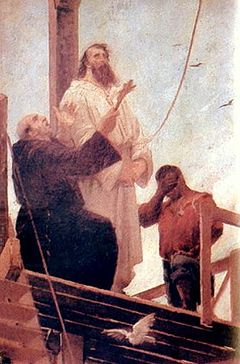
\includegraphics[keepaspectratio]{./images/240px-figueiredo-mhn-tiradentes.jpg}}

O Brasil da República precisava de um herói, e, utilizando a estratégia
de tomar um cadáver emprestado, criaram toda a mística ao redor do
arrancador de dentes que lutara pelo Brasil!

No contexto empresarial, uma vez eu peguei um projeto que já existia,
porém estava em baixa, para aproveitar que o fórum já rolava, inserir
novas ideias e mudar este para o caminho que eu imaginava desde o
início! Seria muito mais difícil criar mais um espaço na agenda de um
monte de gerentes para inserir inovações.

No contexto de filmes, mídia e publicações, isso ocorre direto, basta
ver que as versões N de uma franquia conhecida expandem uma história que
já deveria ter terminado: Star Wars, Velozes e Furiosos, etc.

Destaco por exemplo, o Watchmen original de Alan Moore e Dave Gibbons.
De início, os personagens (Coruja, Comediante, Dr.~Manhattan) eram
heróis bem meia boca provindos de direitos autorais comprados junto à
uma editora antiga, a Carlton Comics.
\pandocbounded{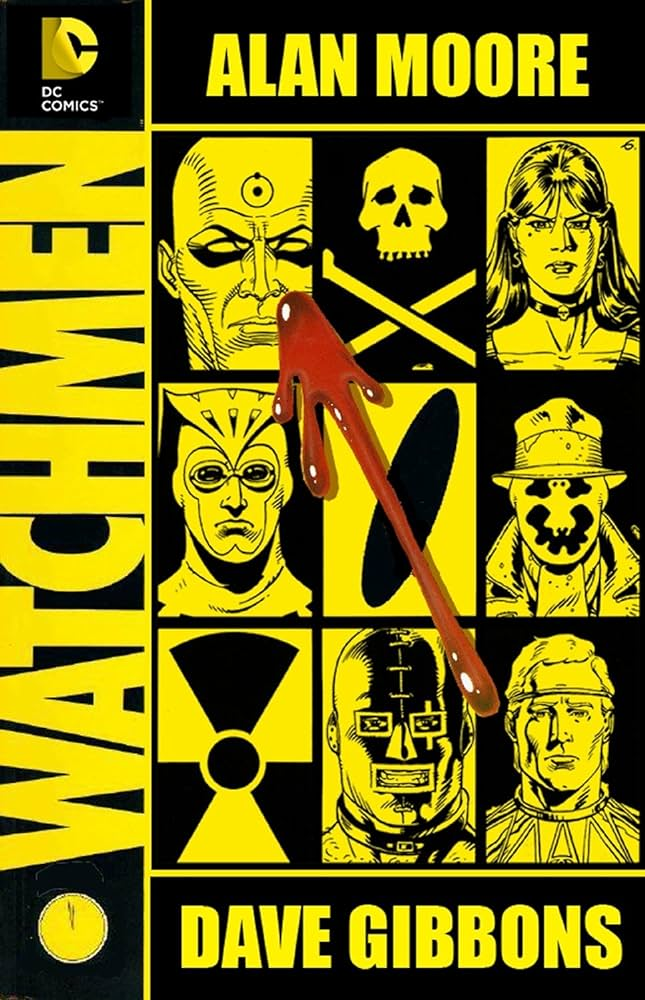
\includegraphics[keepaspectratio]{./images/watchmen.jpg}}

Na mão de Moore e Gibbons, este virou um dos maiores clássicos cult dos
quadrinhos de todos os tempos!

Lembre-se desta estratégia, no próximo feriado de Tiradentes!

\chapter{Estratégia 15 - Atrair um tigre para fora de sua
toca}\label{estratuxe9gia-15---atrair-um-tigre-para-fora-de-sua-toca}

Um tigre é muito forte em seu estado natural, mas vai se retrair em
ambiente desconhecido. Imagine um tigre no deserto, ao invés da
floresta\ldots{}

\pandocbounded{
\includegraphics[keepaspectratio]{./images/Tigre.png}}

Uma estratégia de negociação é chamar o outro lado para uma reunião, e
colocar muita gente do seu time por muito tempo para fazer pressão em
cima do oponente.

Para quem gosta de futebol, um tigre fora de sua toca é como jogar fora
de casa, com a torcida contra, com os gandulas contra, com todo o
ambiente desfavorável.

Estando em seu território, é possível projetar poder. Neste encontro de
Xi Jinping e Trump, em 2026, o assento do norte-americano ``afunda''
mais, o que coloca o seu par chinês numa posição maior. Estratégia assim
já foi utilizada inúmeras vezes.

\pandocbounded{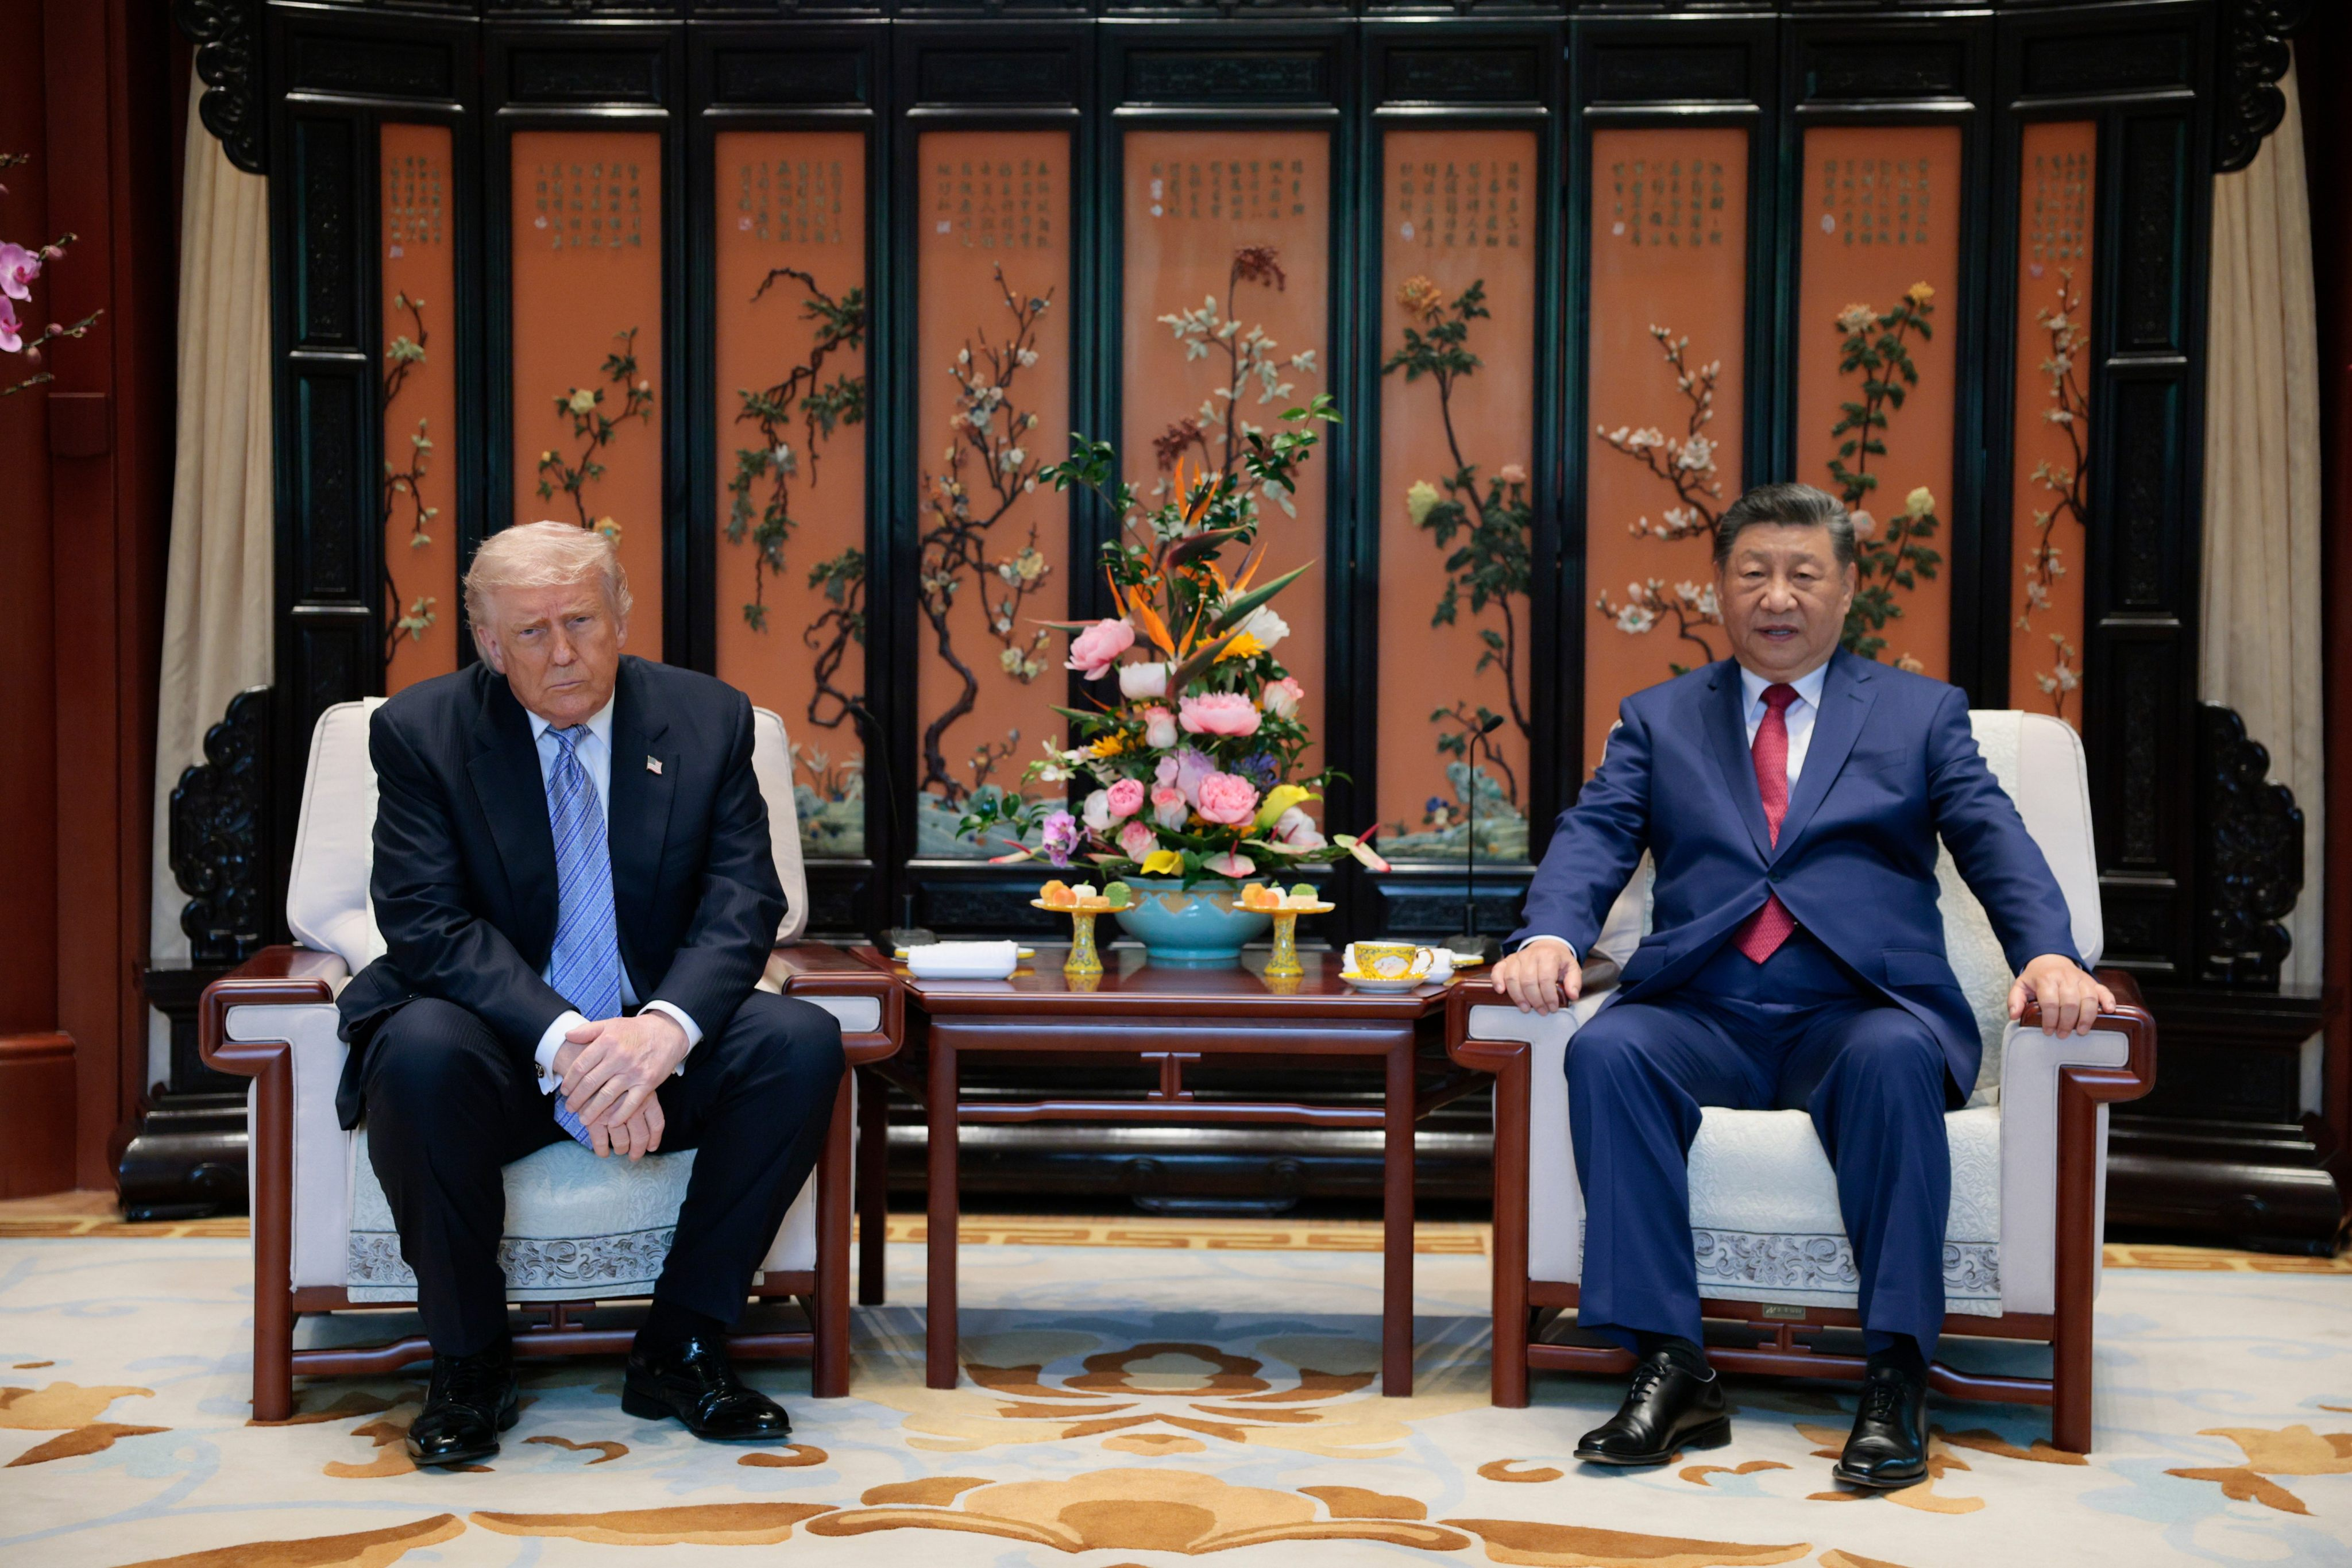
\includegraphics[keepaspectratio]{./images/trump_xi.jpg}}

E como fazer o tigre sair da montanha? Que tal oferecer alguma coisa
para ele vir? Ou marcar num território supostamente ``neutro'', e
conveniente a ambos? Muitas vezes, um simples convite é suficiente.

Algumas variações: chamar o chefe para almoçar quando quiser pedir
aumento, é melhor do que no escritório dele. Levar a sua paquera para um
lugar especial, a fim de pedi-la em casamento.

Esse tema também lembra o belo poema ``The Tiger'' de William Blake:

\pandocbounded{
\includegraphics[keepaspectratio]{./images/Tigre02.png}}

Tiger, tiger, burning bright, In the forest of the night, What immortal
hand or eye Could frame thy fearful symmetry?

\chapter{Estratégia 16 - Soltar um inimigo para recapturá-lo
depois}\label{estratuxe9gia-16---soltar-um-inimigo-para-recapturuxe1-lo-depois}

Há situações em que é melhor não encurralar o inimigo, e sim soltar e
perseguir de perto até este se cansar.

\pandocbounded{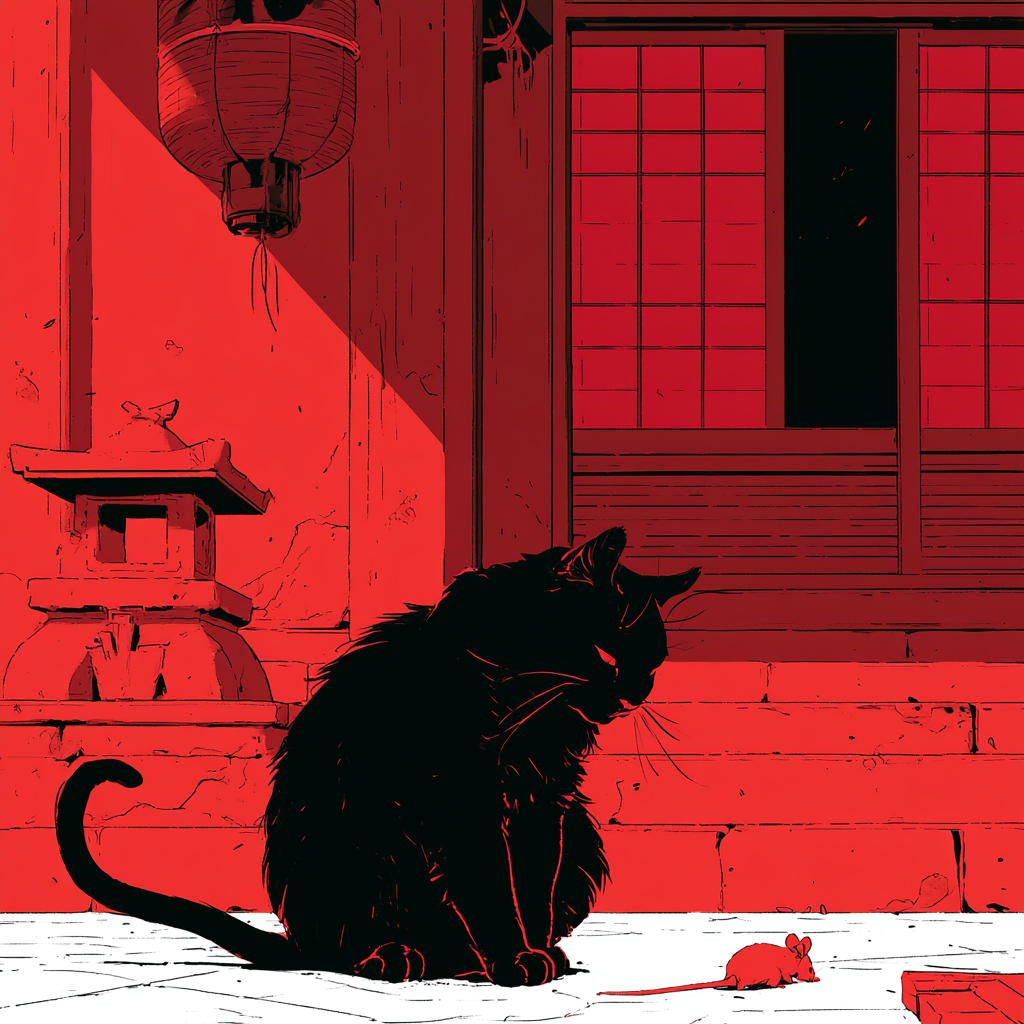
\includegraphics[keepaspectratio]{./images/cat_playing_with_a_mouse.png}}

O filho rebelde só vai entender o que você diz se ele mesmo tentar e
quebrar a cara. Melhor deixar fazer, colocando limites saudáveis, e
esperar que ele mesmo chegue às conclusões.

Numa pescaria, puxar bruscamente o peixe vai fazer a linha arrebentar. É
melhor tensionar e liberar seguidas vezes, até o peixe esgotar suas
forças.

\pandocbounded{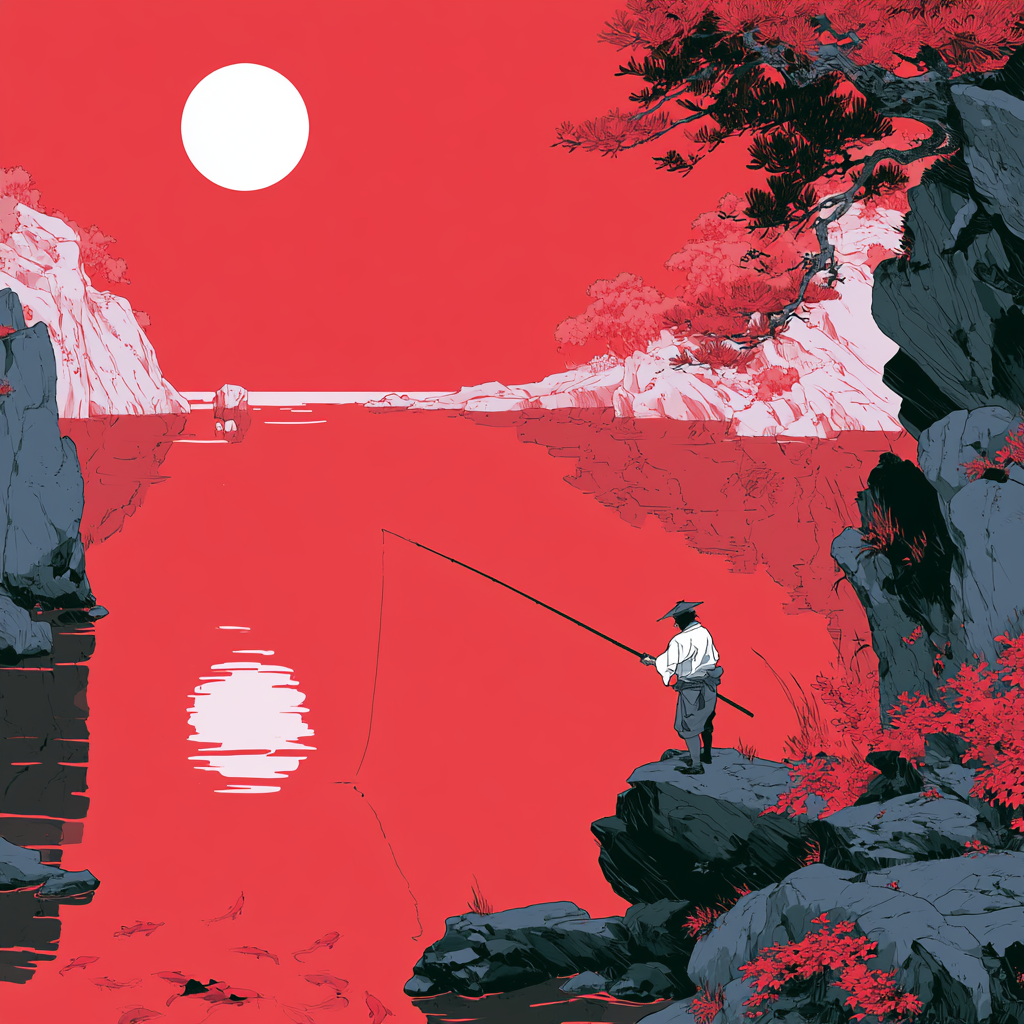
\includegraphics[keepaspectratio]{./images/man_fishing_in_a_lake.png}}

\section{Exemplo. Recapturado e solto 7
vezes}\label{exemplo.-recapturado-e-solto-7-vezes}

Qual a melhor forma de tratar um sujeito obstinado, que não vai desistir
de jeito nenhum?

A história a seguir conta como Zhuge Liang Kongming prendeu e libertou o
líder rebelde Meng Huo 7 vezes.

Zhuge Liang é considerado um dos maiores estrategistas da história da
China, e diversas de suas histórias já foram relatadas neste espaço.

\pandocbounded{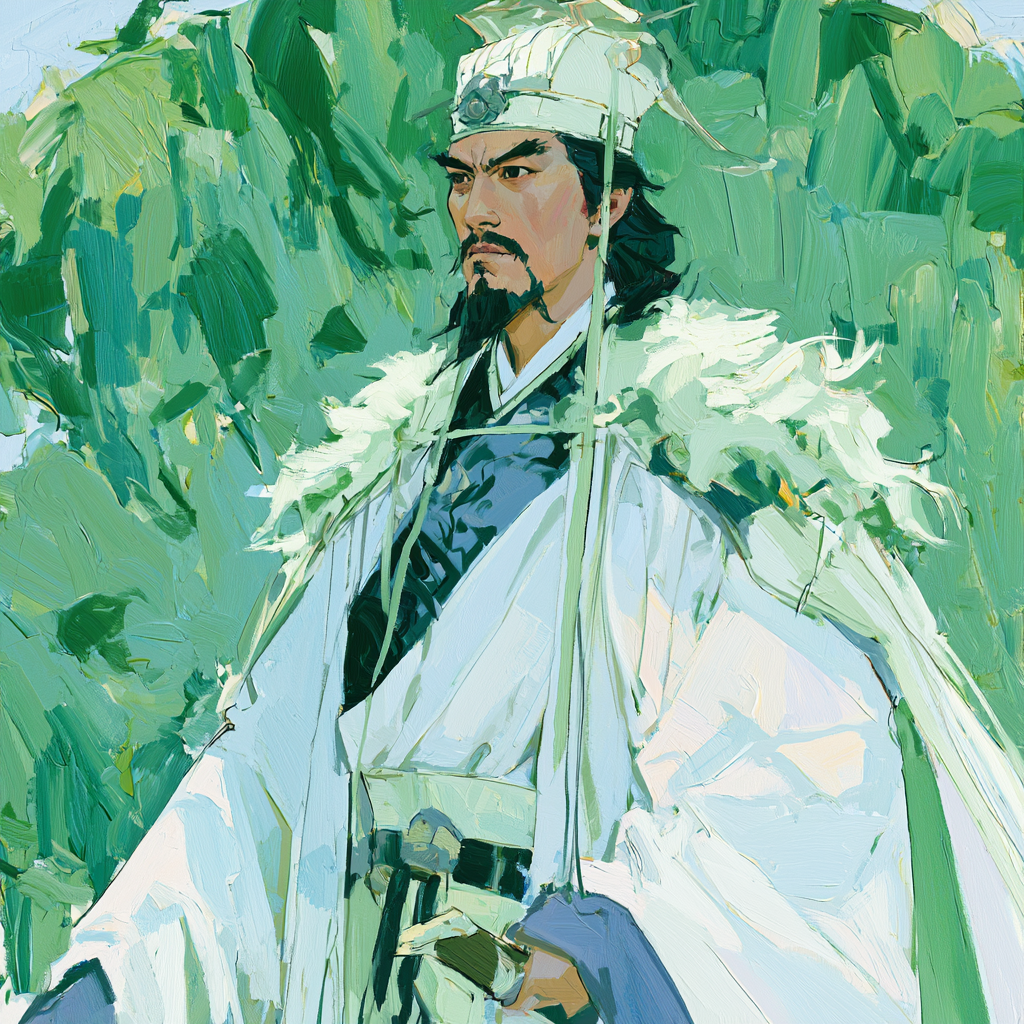
\includegraphics[keepaspectratio]{./images/zhuge_liang_kong_ming.png}}

Meng Huo era um líder carismático, todo o povo rebelde poderia ser
facilmente submetido à sua vontade. Na história dos Três Reinos, Meng
Huo atacou Zhuge Liang, que o derrotou para o libertar em seguida. Meng
Huo atacou de novo, de novo, de novo, tentando diversas estratégias
diferentes, com diversos aliados diferentes. Em todas as oportunidades,
foi mal sucedido, caindo em armadilhas preparadas por Zhuge Liang, que o
capturava para em seguida libertá-lo.

Zhuge Liang poderia facilmente ter eliminado o rebelde em qualquer das 7
vezes que o derrotou, entretanto, isto não traria o fim da guerra.
Talvez, até piorasse. Primeiro, porque outros tomariam o seu lugar, e a
cada vez que ele derrubasse um líder, haveria mais e mais ressentimento
por parte do povo rebelde. Ao invés disso, Zhuge Liang permitiu que o
oponente reorganizasse suas forças e atacasse novamente e novamente.
Continuas vezes derrotado, o líder rebelde finalmente percebeu que não
era páreo para o oponente, e se rendeu. Passou a usar o seu poder de
persuasão sobre o povo e sua habilidade política para coexistir com o
oponente. Não houve mais guerra.

Portanto, há momentos em que, ao invés de prender de forma absoluta, é
melhor deixar ir e voltar.

\chapter{Estratégia 17 - Dar tijolo para obter
jade}\label{estratuxe9gia-17---dar-tijolo-para-obter-jade}

Abrir mão de algo de pouco valor, para obter algo de muito valor.

\pandocbounded{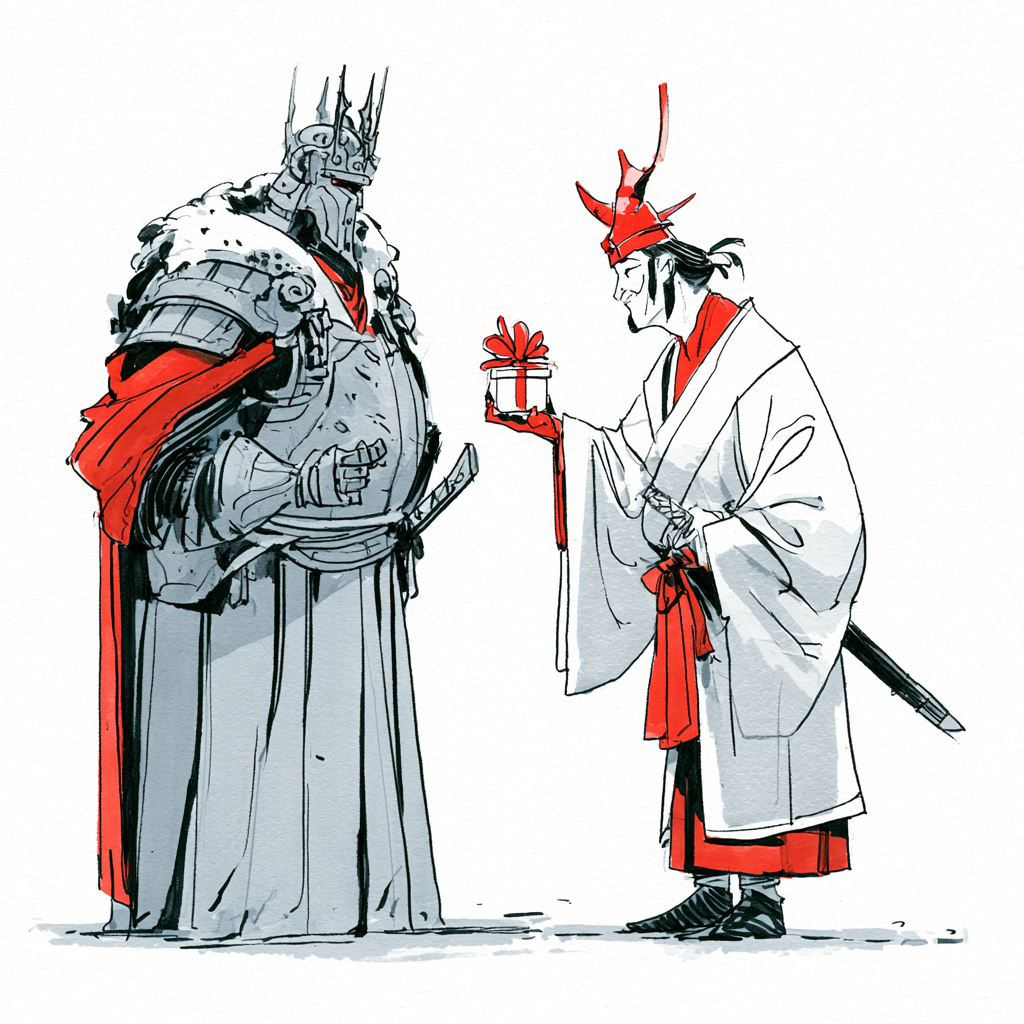
\includegraphics[keepaspectratio]{./images/tijolo_jade.png}}

O comércio tem dezenas de casos assim. A amostra grátis de biscoito,
café, doce, que algum atendente te oferece e você se sente impelido a
comprar um pacote todo, por educação. A revista que você ganha de brinde
enquanto tentam te empurrar a assinatura. A aula gratuita ou um e-book
que é apenas uma introdução para um curso completo, muito mais caro. O
``frete grátis'', o desconto ao comprar mais de um produto, etc\ldots{}

Outra estratégia comum é dar de brinde algum produto encalhado, para
aumentar o valor do produto premium. Ou algo de menos valor, mais
difícil e improvável de resgatar, como milhas de cartão de crédito ou
milhas de companhia aérea. Embora haja alguns aficionados por milhas, a
verdade é que o seu esforço é melhor empregado na sua ocupação principal
do que em estratégias para juntar milhas.

\section{Reciprocidade na
negociação}\label{reciprocidade-na-negociauxe7uxe3o}

A Reciprocidade é uma das estratégias de negociação de Robert Cialdini,
no livro ``Influência''. Naturalmente tendemos a retribuir o que nos é
dado. Então, forneça algo, de pouco ou menor valor, para obter algo de
maior valor. Exemplos citados: Ao receber um cartão de Natal sentimos na
obrigação de enviar também. O pessoal da organização Hare Krishna dá uma
flor ou livro aos viajantes num aeroporto, antes de pedir por doações.
Quem aceitar a flor estará mais propenso a doar também, como
reciprocidade.

\pandocbounded{
\includegraphics[keepaspectratio]{./images/sakura.png}}

O antídoto: Sabendo que existe essa estratégia, não aceitar itens de
pouco valor, ou contra-atacar fornecendo também um item de pouco valor.

\chapter{Estratégia 18 -- Capturar o líder dos
bandidos}\label{estratuxe9gia-18-capturar-o-luxedder-dos-bandidos}

Quando o centro de gravidade orbitar fortemente no líder, e este for
capturado, a organização toda irá desmoronar.
\pandocbounded{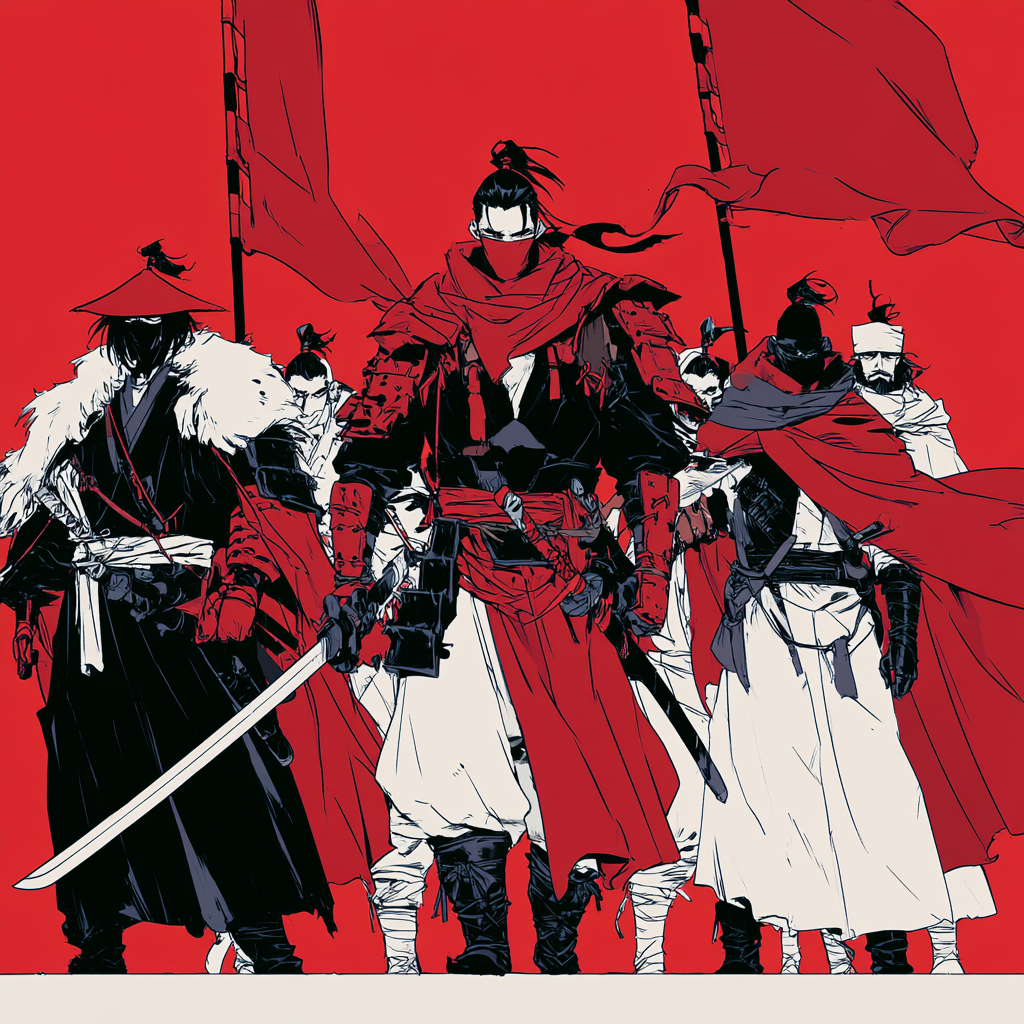
\includegraphics[keepaspectratio]{./images/leader_bandits.png}}

Sendo o líder o pilar que une e guia o time, é natural que afetar este
bagunce todo o restante da organização.

Note o que acontece com todo time que está perdendo: troca o técnico. A
troca do líder gera uma esperança de curto prazo na torcida, de que esta
vez será diferente (mas dificilmente ocorre mudança assim, se não
consertar os problemas estruturais de longo prazo).

Em 2026, o governo americano utilizou esta estratégia para capturar
Nicolas Maduro, ditador venezuelano. Se contou ou não com o apoio local,
não se sabe, porém é fato que o vácuo deixado pelo líder ajuda na
transição para um outro governo.

\pandocbounded{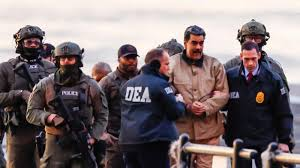
\includegraphics[keepaspectratio]{./images/Maduro.jpeg}}

Sobre o líder, já dizia Sun Tzu: ``O general é a estrela guia do povo, o
senhor de sua segurança e de seu destino''.

Na Apple, por volta de 1985, Steve Jobs estava em pé de guerra com John
Sculley. O Macintosh não tinha dado tão certo assim. Sculley,
pragmático, queria uma empresa mais saudável operacionalmente, deixando
de lado a veia inovativa de Jobs.

Sculley faria uma viagem à China, à trabalho.

Jobs viu nisso uma oportunidade. Ele planejou convencer o conselho a
remover Sculley enquanto ele estivesse fora do país. A ideia era
reorganizar a Apple e retomar o controle da companhia.
\pandocbounded{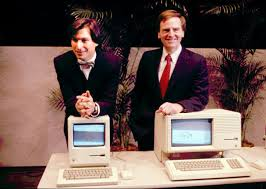
\includegraphics[keepaspectratio]{./images/jobs_sculley.jpeg}}

A estratégia não deu certo. O plano vazou, Sculley cancelou a viagem, e,
por fim, foi Jobs quem deixou a empresa.

Algumas décadas depois, no icônico discurso de formatura de Stanford em
2011, Steve Jobs disse, em relação à sua saída da Apple:

``Tenho certeza de que nada disso teria acontecido se eu não tivesse
sido demitido da Apple. Foi um remédio horrível, mas eu entendo que o
paciente precisava. Às vezes, a vida bate com um tijolo na sua cabeça.
Não perca a fé. Estou convencido de que a única coisa que me permitiu
seguir adiante foi o meu amor pelo que fazia. Você tem que descobrir o
que você ama. Isso é verdadeiro tanto para o seu trabalho quanto para
com as pessoas que você ama.''

\part{19 a 24}

\chapter{Estratégias de Confusão}\label{estratuxe9gias-de-confusuxe3o}

Compreendem as estratégias de 19 a 24.

\pandocbounded{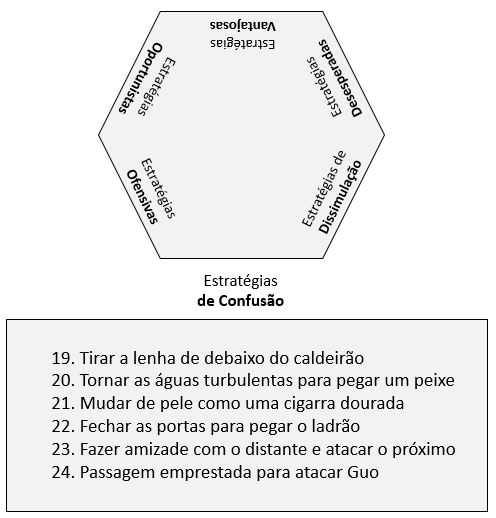
\includegraphics[keepaspectratio]{./images/36strategies_4.jpg}}

\href{estrategia_19.qmd}{19 -- Tirar a lenha de debaixo do caldeirão.}

\href{estrategia_20.qmd}{20 -- Tornar as águas turbulentas para pegar um
peixe.}

\href{estrategia_21.qmd}{21 -- Mudar de pele como uma cigarra dourada.}

\href{estrategia_22.qmd}{22 -- Fechar as portas para pegar o ladrão.}

\href{estrategia_23.qmd}{23 -- Fazer amizade com o distante e atacar o
próximo.}

\href{estrategia_24.qmd}{24 -- Passagem emprestada para atacar Guo.}

\chapter{Estratégia 19 -- Tirar a lenha de debaixo do
caldeirão}\label{estratuxe9gia-19-tirar-a-lenha-de-debaixo-do-caldeiruxe3o}

Ao invés do confronto direto, utilizar táticas para minar a moral do
inimigo.

Retire a lenha, para evitar que a água ferva, corte a grama destruindo
as raízes.

\pandocbounded{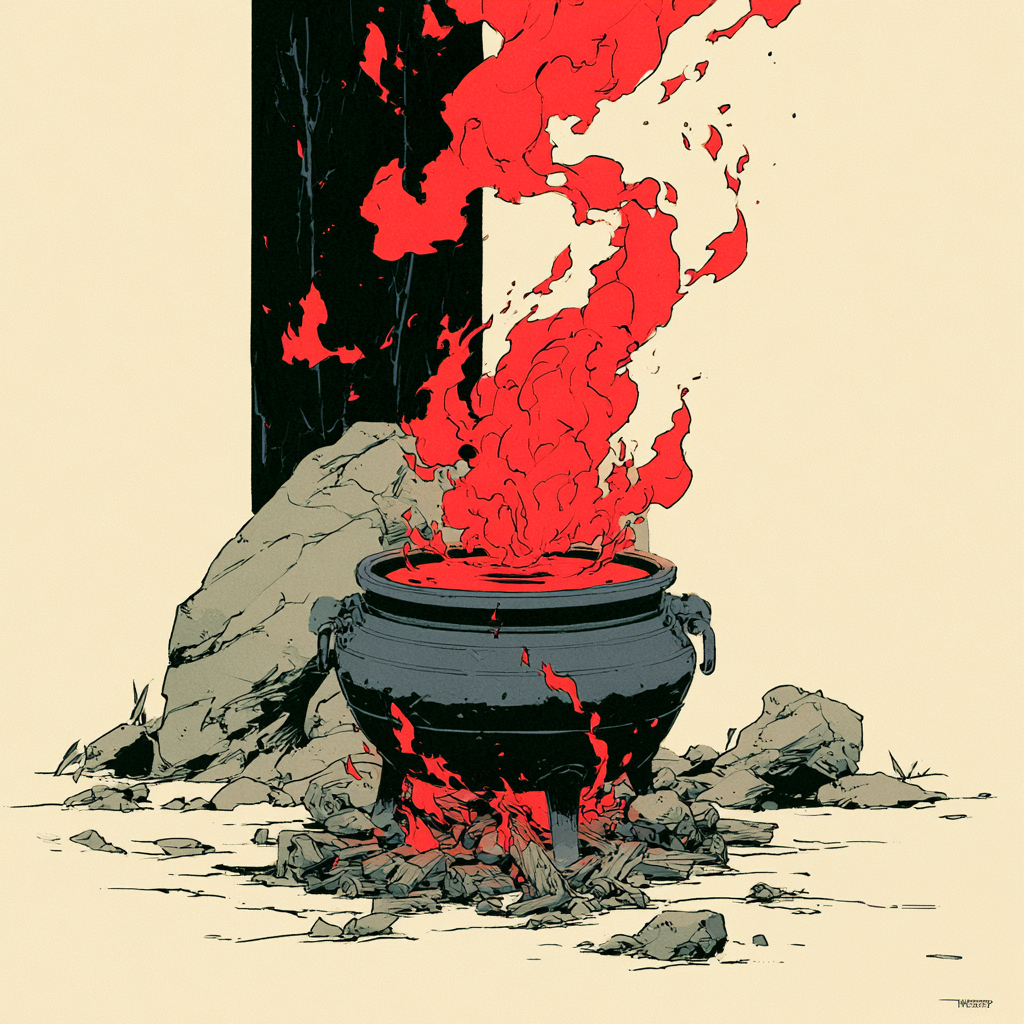
\includegraphics[keepaspectratio]{./images/lenha_fogueira.png}}

A estratégia vem da seguinte história.

O grande Confúcio era conselheiro do imperador de Lu, o que fazia com
que este tivesse força e sabedoria. A fim de atacar Lu, o inimigo
primeiramente tirou Confúcio da jogada. Ele fez oferendas de ouro,
presentes, bebidas, cavalos e oitenta beldades para o imperador de Lu.
Este aceitou as oferendas e passou a levar uma vida de libertinagem,
ignorando Confúcio, que pediu exoneração do cargo meses depois. Sem a
sabedoria de Confúcio, o império Lu foi facilmente manipulado e
conquistado, anos depois.

Se, na estratégia 18, a ideia era atacar o líder, nesta é atacar o seu
suporte.

Numa negociação, às vezes o diretor da área não tem conhecimento técnico
o suficiente para discernir entre soluções. Então, é a pessoa técnica do
seu time é que deve ser convencida e, aí sim, esta convencerá o diretor
sobre o rumo a tomar.

Um time de futebol que tem apenas atacantes bons, mas não o meio-campo,
nunca se destacará em nada.

Nas empresas, nesses tempos atuais de ``eficiência operacional'' e corte
de custos, é perigoso tirar a lenha do caldeirão de si mesmo e o corte
ter consequências péssimas.

É como uma aranha, que tem oito patas.

\pandocbounded{
\includegraphics[keepaspectratio]{./images/spider.png}}

Você tira uma pata, a título de ``eficiência operacional'', ``fazer mais
com menos'' e ela continua andando. Tira duas patas, três, até que chega
uma hora que\ldots{} ela não aguenta mais, e ela tomba.

Cuidado para não retirar lenha do seu próprio caldeirão!

\chapter{Estratégia 20 -- Tornar as águas turbulentas para pegar um
peixe}\label{estratuxe9gia-20-tornar-as-uxe1guas-turbulentas-para-pegar-um-peixe}

Fazer um lamaçal para o peixe ficar confuso e capturá-lo. Um exército
confuso proporciona a vitória ao inimigo.

\pandocbounded{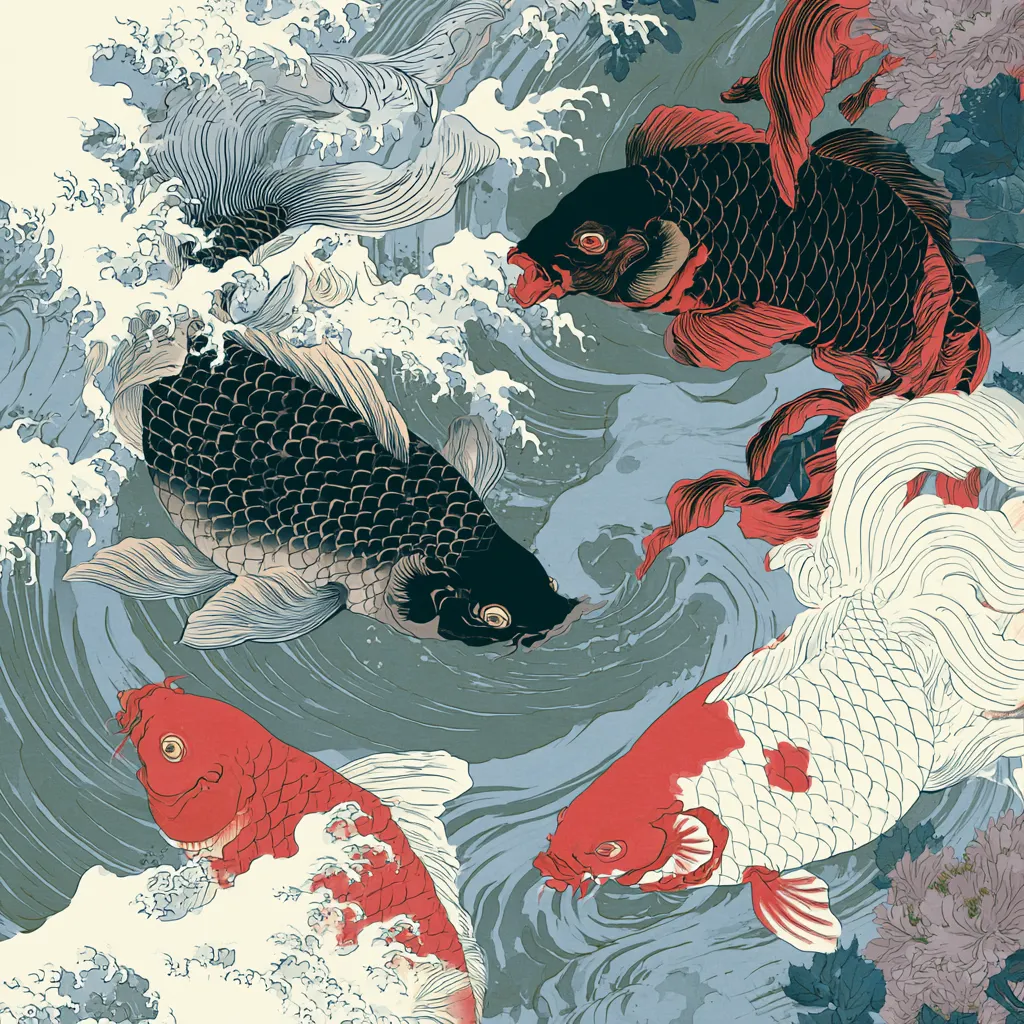
\includegraphics[keepaspectratio]{./images/fish.png}}

A tática de criar ruído é comumente utilizada. Quando uma área não quer
fazer um trabalho, ela pode levantar uma série de objeções, como
problemas legais, necessidade de maior estudo, mensurar melhor as
``dores do problema'' e assim sucessivamente.

Em 496 a.C. as tropas do reino de Yue fizeram uma manobra inesperada,
numa batalha contra o reino de Wu. Uma fileira de soldados de Yue
marchou à frente, desembainhou as espadas e cortou as próprias
gargantas.

\pandocbounded{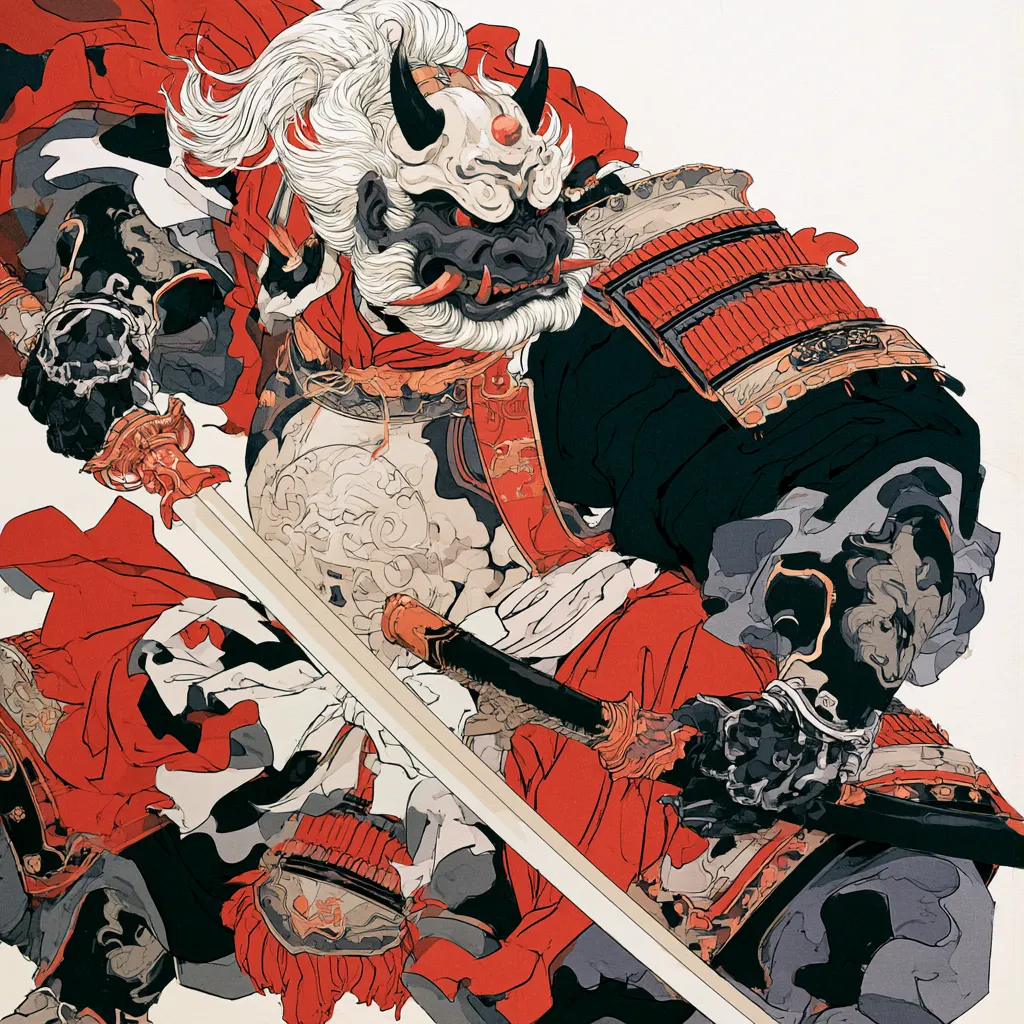
\includegraphics[keepaspectratio]{./images/chinese_warrior_with_a_demon.png}}

Sem entender absolutamente nada do que ocorrera, as tropas inimigas
entraram em choque, possibilitando um momento de confusão e de ataque
concentrado do primeiro. Mal eles sabiam que a tropa suicida era de
condenados à morte, e que tinham duas opções: cometerem tal suicídio
espantoso ou serem executados pelas tropas de Yue.

No Xadrez, mesmo numa posição perdida, quando o oponente ataca por um
lado, você contra-ataca pelo outro lado, ou pelo centro. Ou coloca uma
peça importante, como uma torre, como um alvo atacável no outro flanco.

De forma geral, o lado que estiver em desvantagem deve tentar fazer
alguma coisa para tumultuar o ambiente, distrair o adversário. Já, quem
estiver em posição vantajosa, deve focar no que interessa e ignorar
distrações.

O blefe pode dar certo ao distrair a atenção do oponente.

Algumas dicas para evitar a confusão: Canais de comunicação eficientes
Procedimentos claros Feedback preciso

Outra interpretação possível deste estratagema diz respeito à isca. O
peixe é alvo que queremos obter, e pela analogia da pesca, temos a isca.

\pandocbounded{
\includegraphics[keepaspectratio]{./images/wonderful_gorgeous_woman.png}}

Seja dinheiro, poder, influência, sexo oposto, há algo na isca que atrai
a atenção do alvo.

Dizem os livros antigos, que ``Pega-se o peixe pequeno com uma linha
fina e isca visível; o peixe médio com uma linha proporcional e uma isca
apetecível; o peixe grande com uma linha grossa e uma isca grande. Com o
homem, é o mesmo.''

\chapter{Estratégia 21 - Mudar de pele como uma cigarra
dourada}\label{estratuxe9gia-21---mudar-de-pele-como-uma-cigarra-dourada}

Escapar sem ser percebido, como a cigarra que muda de pele. Utilizar uma
pele específica segundo a circunstância. Adaptar-se à mudanças que
ocorrem constantemente no meio-ambiente.

\pandocbounded{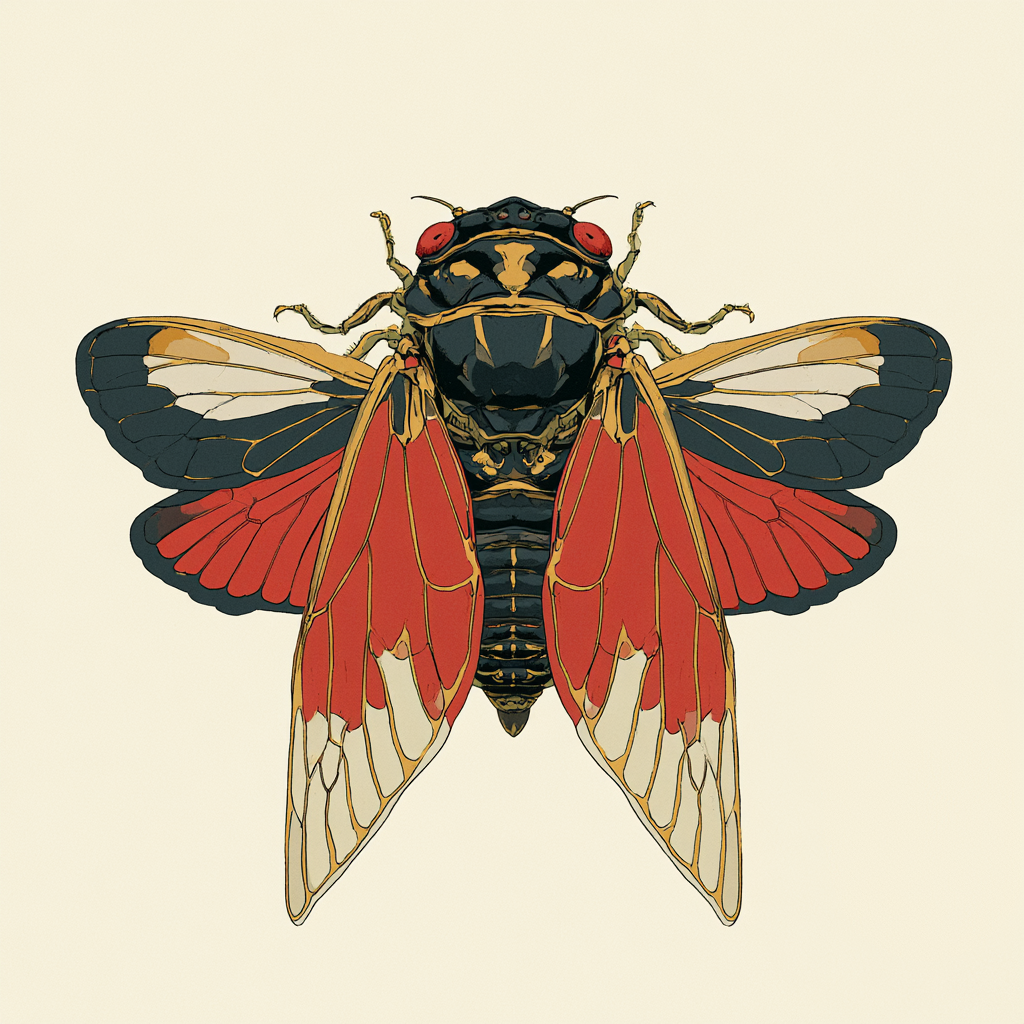
\includegraphics[keepaspectratio]{./images/golden_cicada.png}}

Há pessoas que são, naturalmente, mestres nisso. Mudam de opinião
conforme o chefe muda de humor. Autêntico ``Maria-vai-com-as-outras''.

O grande guerreiro da época dos Três Reinos, Lu Bu, era um hóspede /
prisioneiro incômodo no reino de Shao.

\pandocbounded{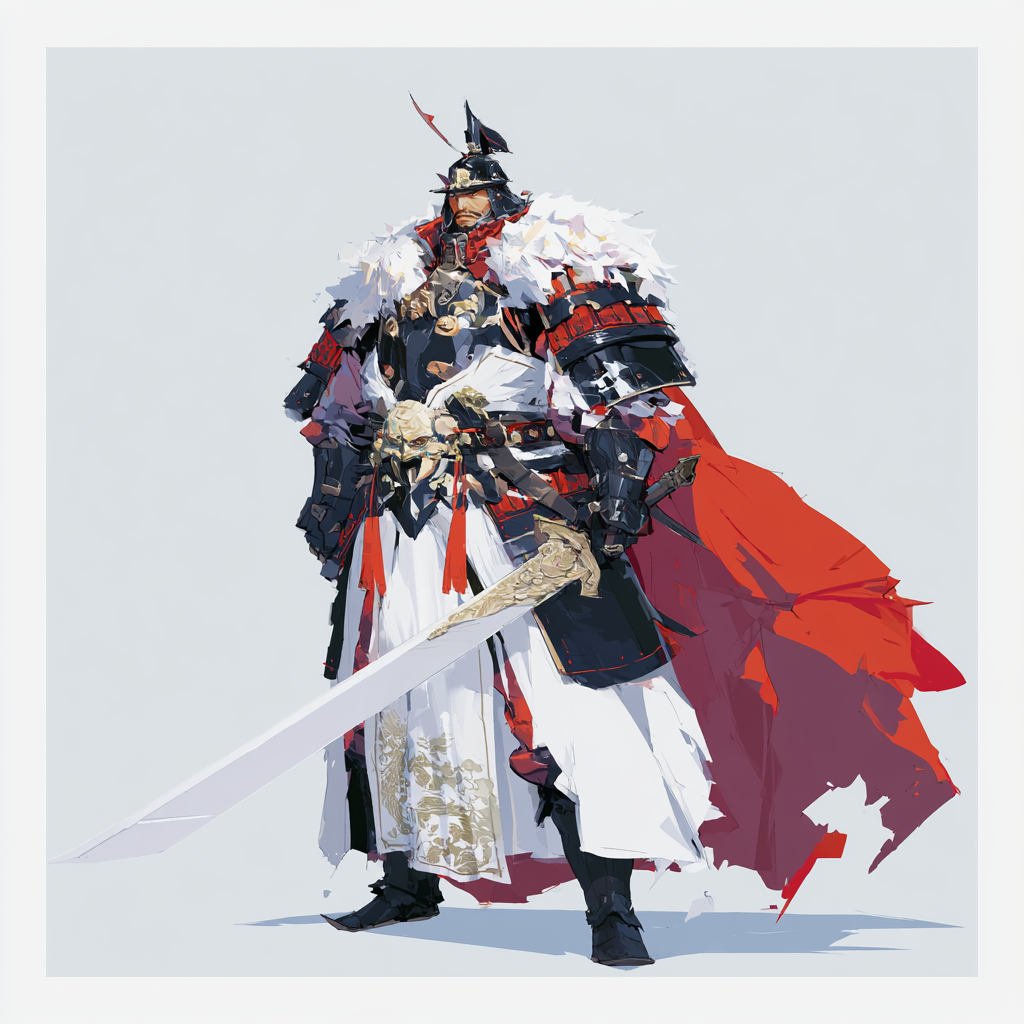
\includegraphics[keepaspectratio]{./images/Lu_Bu.png}}

Um dia, o Rei de Shao liberou Lu Bu para retornar ao seu Estado, porém,
logo achou que estaria ``devolvendo um tigre à montanha''. Lu Bu era
perigoso demais para ficar vivo. Enviou junto uma tropa de 30 homens,
com o pretexto de ser uma escolta para o guerreiro.

À noite, Lu Bu convidou um de seus comandantes para jogar um jogo de
tabuleiro. Ficaram em sua tenda, por horas, até que luz da tocha se
apagasse.

Quando os soldados de Shao entraram na tenda para proceder à execução,
encontraram apenas um boneco de pano e algodão. Lu Bu fugira, há tempos!

Um episódio famoso da Segunda Grande Guerra foi o pacto de não agressão
entre Alemanha e União Soviética. Hitler e Stalin se odiassem mutuamente
e todos sabiam que era um pacto temporário. Uma questão de tempo até que
um dos dois descumprisse o acordo.

\pandocbounded{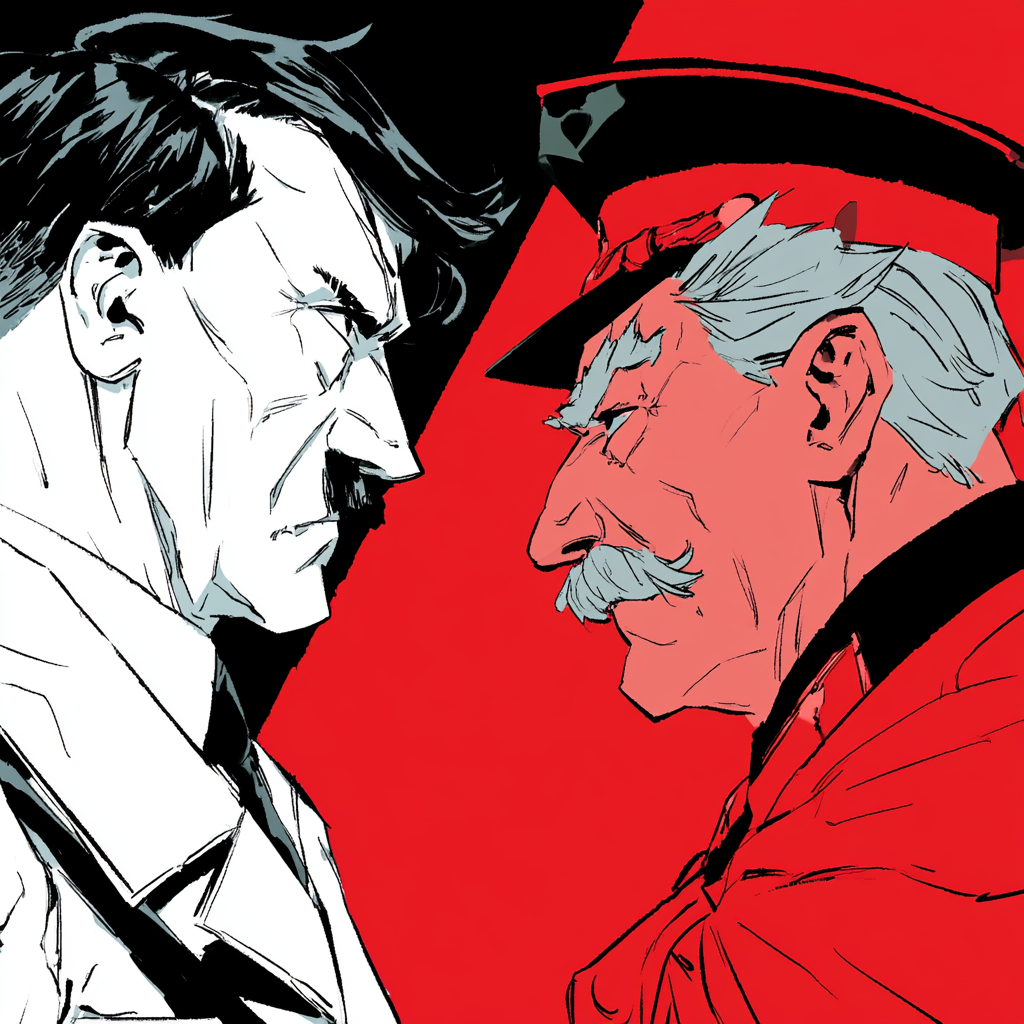
\includegraphics[keepaspectratio]{./images/hitler_against_stalin.png}}

O tempo ganho foi utilizado para a Alemanha focar em atacar o oeste
europeu (França, Inglaterra), para ambos os pactuantes dividirem a
Polônia, e para a URSS se preparar para a guerra que inevitavelmente
chegaria.

Alguns anos após o pacto, a Alemanha quebrou o tratado e invadiu a URSS.
Stalin ``mudou de pele'' conforme circunstâncias.

Em uma grande empresa, uma forma de mudar a pele é utilizar consultoria.
Para fazer cumprir alguma medida impopular de redução de custos e de
pessoal, ou ratificar alguma estratégia que seria tomada de qualquer
forma, é comum o uso de consultorias, a fim de dar um ar de isenção e
legitimidade técnica. De certa forma, é o outro lado da moeda da
Estratégia 3, de utilizar uma faca emprestada, agora do ponto de vista
do contratante do serviço.

Em âmbito pessoal, mudamos de pele todos os dias. Eu sou uma pessoa
quando trabalhando, ou numa ocasião de negócios. Em casa, com a família
e longe de pressões sociais, posso ``tirar a armadura'' e ser algo mais
próximo de mim mesmo.

\chapter{Estratégia 22 -- Fechar as portas para pegar o
ladrão}\label{estratuxe9gia-22-fechar-as-portas-para-pegar-o-ladruxe3o}

Quando o inimigo é fraco, ele perde o espírito de luta ao se ver cercado
como o ladrão preso na numa casa.

\pandocbounded{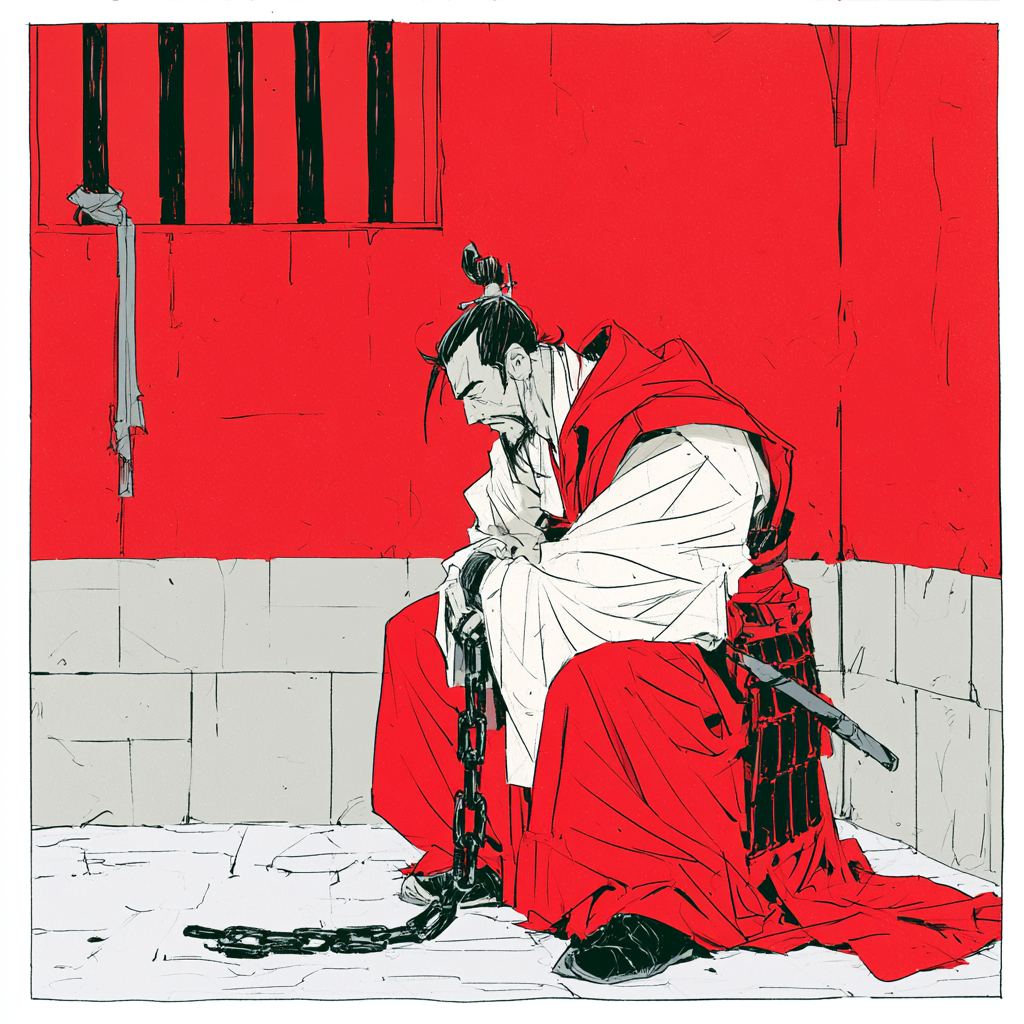
\includegraphics[keepaspectratio]{./images/prisioner.png}}

A estratégia de ``fechar a porta'' pode ser interpretada como fazer um
cerco, privar o adversário de todos os recursos externos.

Cerco a cidades muradas é uma estratégia antiga e muito utilizada.
Tentar furar a proteção de uma cidade murada é difícil, inevitavelmente
levará a enormes baixas. Já o cerco é uma forma indireta de ataque, de
sufocar o inimigo, que vai, lentamente, padecendo. É necessário ter
paciência e determinação para manter o cerco.

Júlio César, o grande general romano, era famoso por utilizar tal
estratégia. Contra os gauleses, por exemplo, foi feito um cerco
prolongado. Após alguns meses, todos os recursos do adversário estavam
exauridos, e eles foram forçados a se renderem.

Júlio César, era um brilhante estrategista, mas os engenheiros dele eram
tão importante quanto os guerreiros, as espadas e as flechas. O exército
romano era capaz de se mover velozmente, abrir estradas, montar cercos e
verdadeiras fortalezas a fim de sobrepujar o inimigo!

\pandocbounded{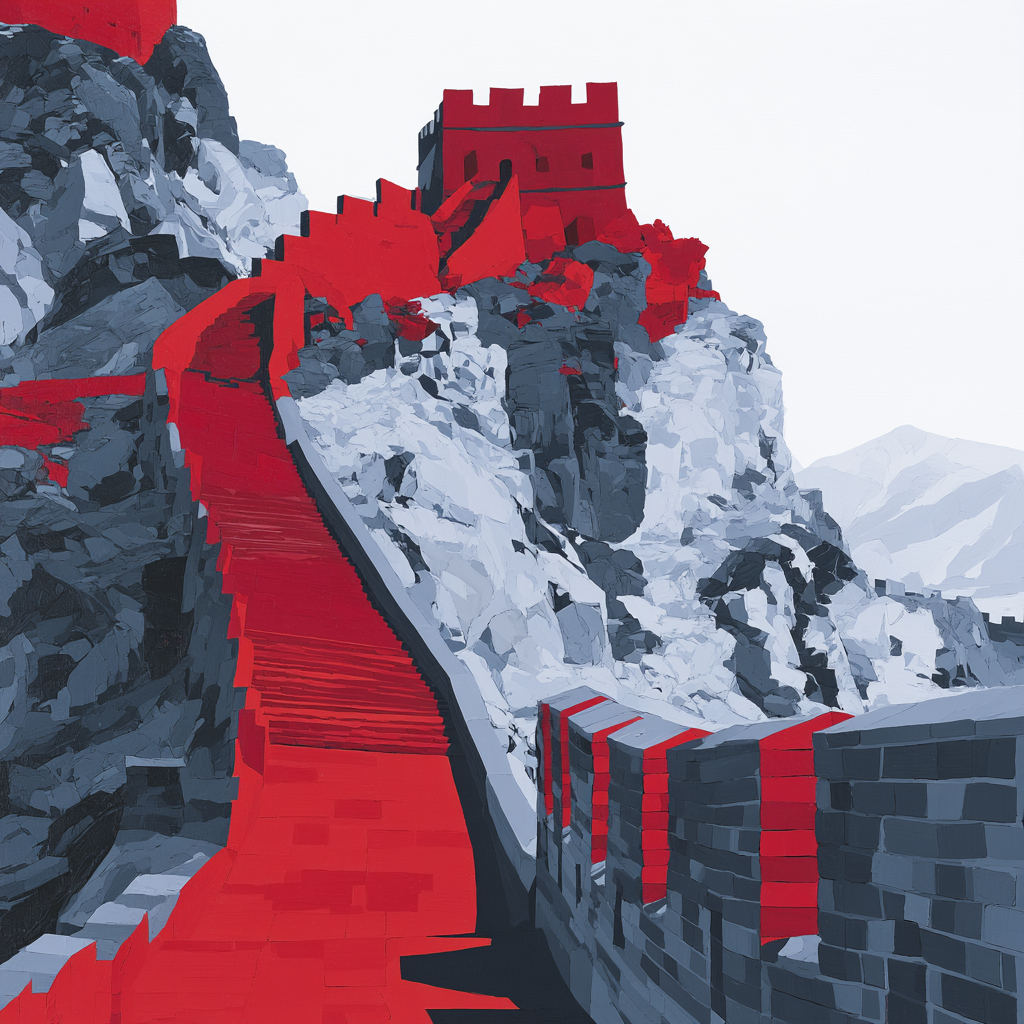
\includegraphics[keepaspectratio]{./images/wall.png}}

Sun Tzu diz ``Se nossas forças forem dez vezes maiores que as do
inimigo, devemos cercá-lo; se cinco vezes maiores, atacá-lo; se duas
vezes maiores, dividi-lo.''

Há ainda outra máxima de Sun Tzu:

``Quando cercar um exército, deixe uma saída livre.''

A ideia é que um inimigo sem esperança luta com desespero. Muitas vezes
é melhor oferecer uma rota de fuga e destruir sua capacidade de
resistência com tal tentação de refúgio, do que oferecer a ele a luta
total como última saída.

No mundo dos negócios, há vários cercos possíveis: barreiras
regulatórias, jurídicas, patentes, conhecimento e pessoas
especializadas. As grandes empresas vivem colocando inúmeras dessas
barreiras, a fim de manter a sua posição frente a concorrentes menores e
mais inovadores.

Para aplicar a estratégia de ``fechar a porta'', é necessário ter uma
força superior em montar e manter a barreira.

\chapter{Estratégia 23 -- Fazer amizade com o distante e atacar o
próximo}\label{estratuxe9gia-23-fazer-amizade-com-o-distante-e-atacar-o-pruxf3ximo}

Formar alianças estratégicas com sócios distantes para atacar um
concorrente local.

\pandocbounded{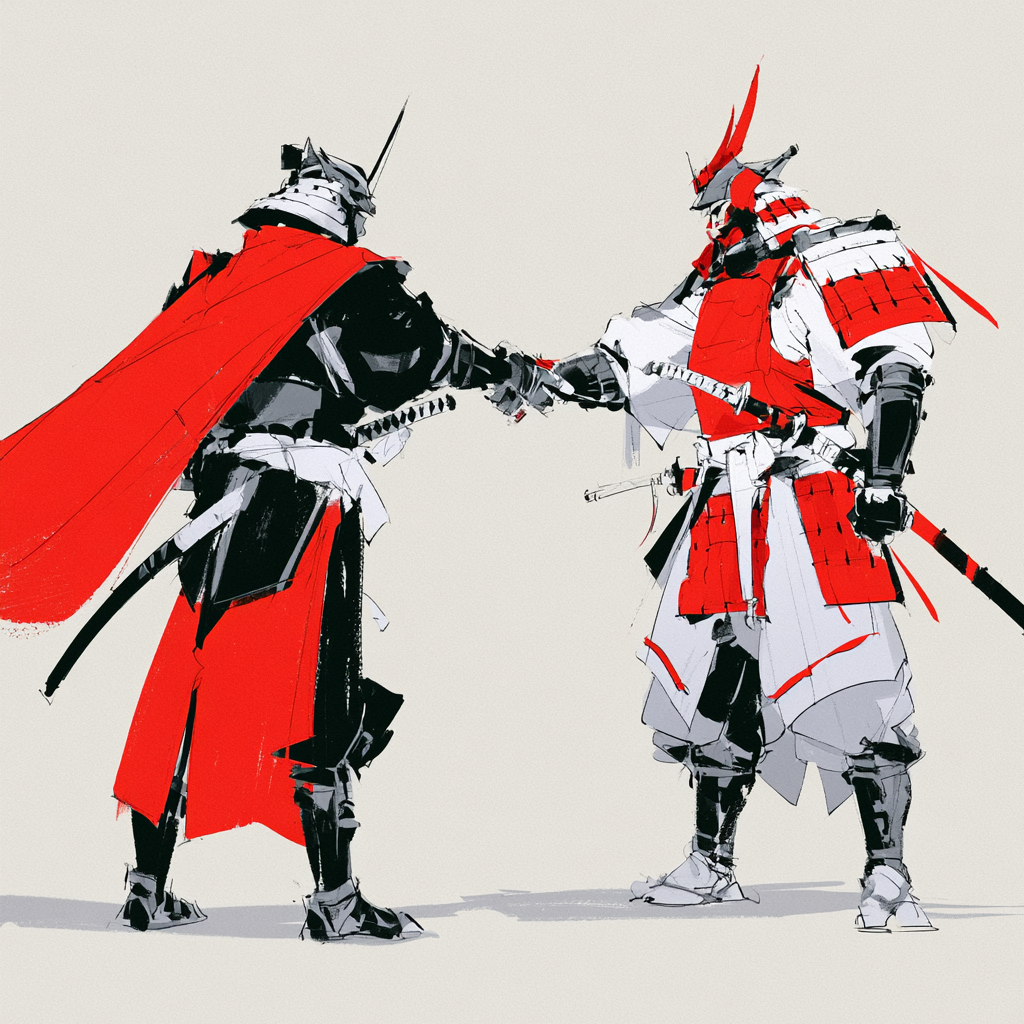
\includegraphics[keepaspectratio]{./images/warriors_shaking_hads.png}}

\begin{verbatim}
Exemplo: uma companhia pode fazer parte de uma aliança internacional com outras companhias, e com isso obter vantagem sobre o concorrente local.
\end{verbatim}

\chapter{Estratégia 24 -- Passagem emprestada para atacar
Guo}\label{estratuxe9gia-24-passagem-emprestada-para-atacar-guo}

Utilizar algum recurso de outrem, como uma passagem por dentro do
território, para atacar o inimigo. Na estratégia 3, matar com uma faca
emprestada, é o terceiro que faz a ação, agora na estratégia 24, sou eu
que faço a ação, e o terceiro apenas empresta recursos.

\pandocbounded{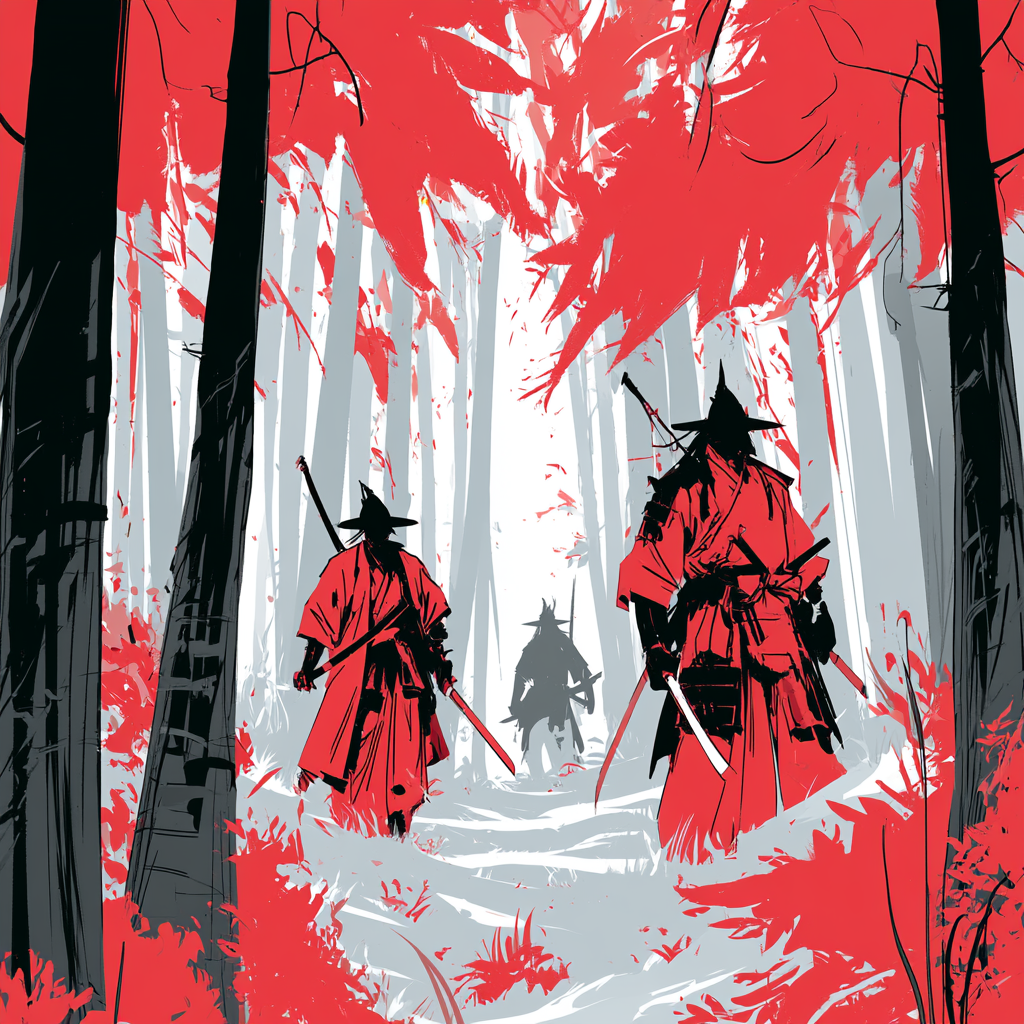
\includegraphics[keepaspectratio]{./images/narrow_path.png}}

Exemplo: vender o seu produto com a marca de outra companhia, para
``pegar emprestado'' o nome desta.

\part{25 a 30}

\chapter{Estratégias de
Dissimulação}\label{estratuxe9gias-de-dissimulauxe7uxe3o}

Compreendem as estratégias de 25 a 30.

\pandocbounded{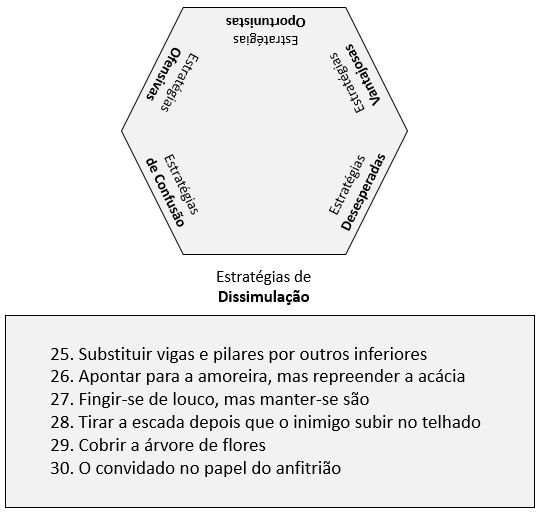
\includegraphics[keepaspectratio]{./images/36strategies_5.jpg}}

\href{estrategia_25.qmd}{25 -- Substituir vigas e pilares por outros
inferiores.}

\href{estrategia_26.qmd}{26 -- Apontar para a amoreira, mas repreender a
acácia.}

\href{estrategia_27.qmd}{27 -- Fingir-se de louco, mas manter-se são.}

\href{estrategia_28.qmd}{28 -- Tirar a escada depois que o inimigo subir
no telhado.}

\href{estrategia_29.qmd}{29 -- Cobrir a árvore de flores.}

\href{estrategia_30.qmd}{30 -- O convidado no papel do anfitrião.}

\chapter{Estratégia 25 -- Substituir vigas e pilares por outros
inferiores}\label{estratuxe9gia-25-substituir-vigas-e-pilares-por-outros-inferiores}

Alterar estruturas importantes, como vigas e pilares, por materiais de
qualidade inferior, e com isso enfraquecer o inimigo.

Exemplo: Uma vez comprei um carro, que tinha uma lataria muito bonita.
Alguns meses depois, problemas começaram a acontecer. O carro ficava
acelerado, por conta de uma pecinha que tinha quebrado. A vidro elétrico
também quebrou. Depois, o para-brisa. Debaixo da aparência, peças
inferiores.

Depois de tal episódio, comprei um Toyota que nunca teve nenhum
incidente. A partir daí, só comprei carros desta marca. Tenho a
confiança de que todas as peças, por menores que sejam, têm um elevado
padrão de qualidade.

É comum times de futebol que têm uma temporada excelente, com titulares
e reservas jogando no topo da capacidade. Aí, na temporada seguinte, as
estrelas titulares saem, reservas viram titulares, e reservas dos
reservas viram os novos substitutos. E, não raro, o desempenho cai
enormemente, só em substituir a base de sustentação por outras peças
menores.

As vigas e pilares são invisíveis, porém, como dizia o Pequeno Príncipe,
``O essencial é invisível aos olhos''.

Se a estratégia 18 era sobre o ``Líder dos bandidos'' e a estratégia 19
``Tirar a lenha de debaixo do caldeirão'', a diferença desta é que as
vigas e pilares estão ainda mais nas fundações, enquanto as estruturas
acima atacam mais o topo.

Um exemplo do mundo corporativo é eliminar postos demais em funções
técnicas e operacionais, sobrecarregando os demais a título de ``ganho
de eficiência''.

\pandocbounded{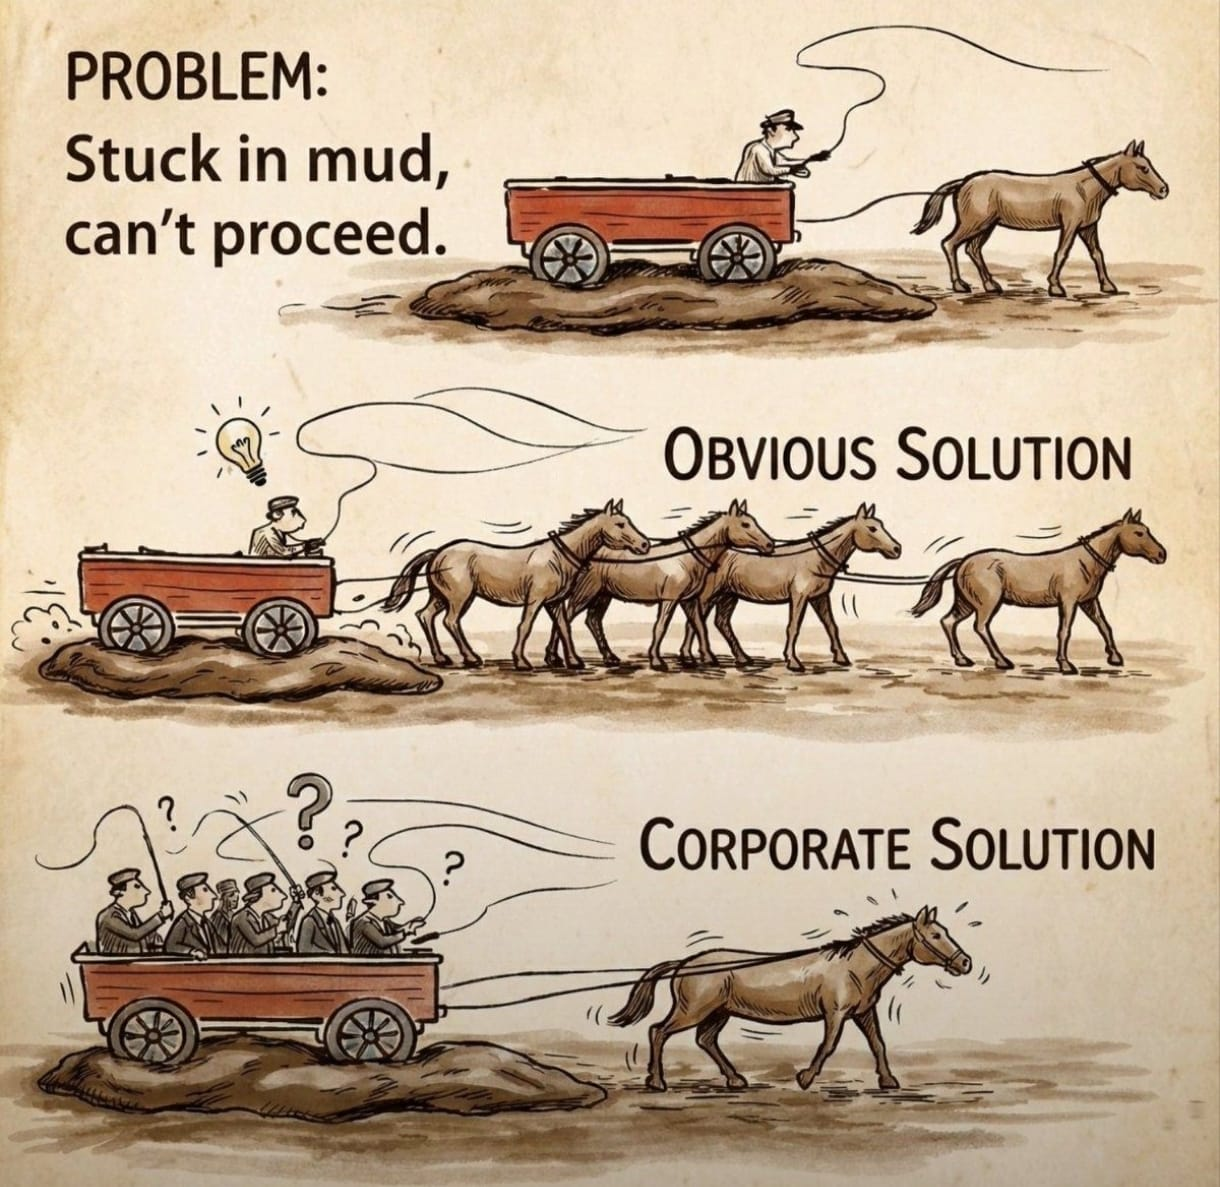
\includegraphics[keepaspectratio]{./images/Meme_corporativo.jpeg}}

Curioso que, frequentemente, os salários e compensações dos altos
executivos só aumentam. Além disso, é comum a contratação de grandes
consultorias, para trazer ``as melhores práticas de mercado'', comumente
aumentando mais ainda a pressão sobre a base\ldots{}

\chapter{Estratégia 26 -- Apontar para a amoreira, mas repreender a
acácia}\label{estratuxe9gia-26-apontar-para-a-amoreira-mas-repreender-a-acuxe1cia}

Consiste em repreender indiretamente, utilizar alguém fraco para mandar
a mensagem para alguém forte. Uma variação desta estratégia é ``Matar a
galinha para assustar o macaco''.

\pandocbounded{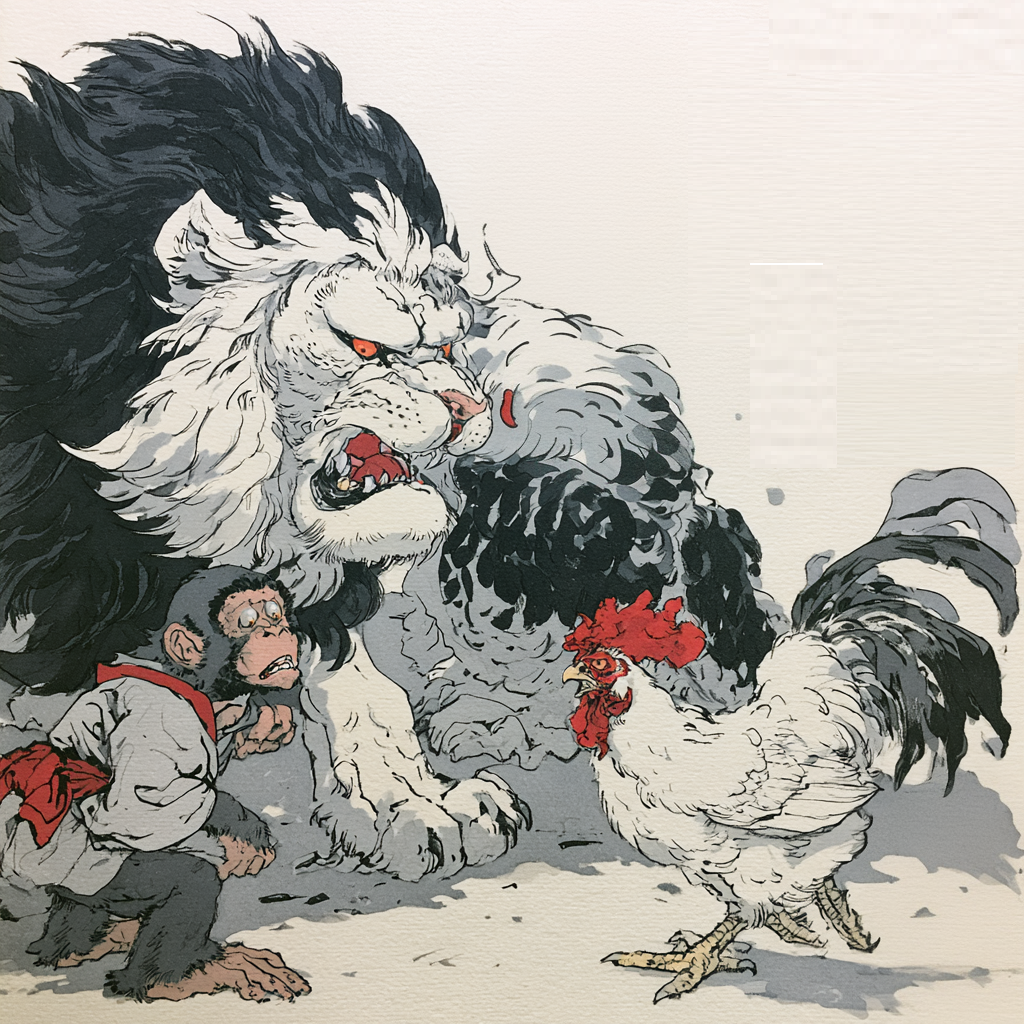
\includegraphics[keepaspectratio]{./images/A_lion_menacing_a_chicken_and_a_afraid_monkey.png}}

A galinha é muito mais fraca do que o macaco, e matar a galinha tem como
objetivo controlar o macaco.

\chapter{Estratégia 27 -- Fingir-se de louco, mas manter-se
são}\label{estratuxe9gia-27-fingir-se-de-louco-mas-manter-se-suxe3o}

É melhor fingir que não sabe e não tomar providência do que fingir que
sabe tudo e se meter em um situação que não é possível contornar. Melhor
fingir-se tolo numa situação difícil e se preparar para um momento
posterior.

\pandocbounded{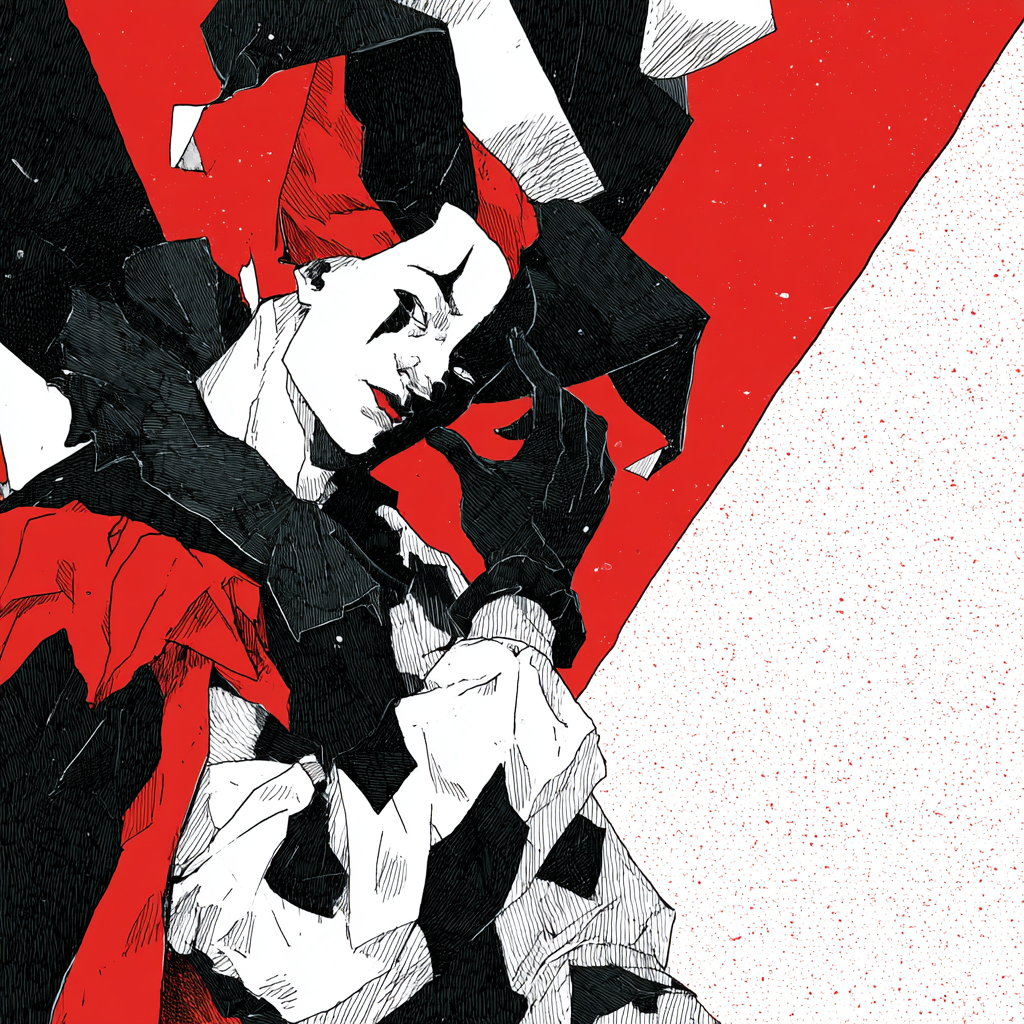
\includegraphics[keepaspectratio]{./images/fool.png}}

O imperador romano Cláudio era figura pouco destacada. Era coxo e gago.
Não demonstrava nenhuma aptidão política.

\pandocbounded{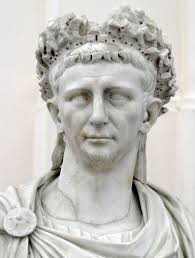
\includegraphics[keepaspectratio]{./images/claudio.jpeg}}

Quando os legionários assassinaram o seu predecessor Calígula,
encontraram Cláudio escondido atrás de uma cortina. Cláudio foi poupado,
porque parecia bobo, inepto, daria um imperador fantoche perfeito.

Mas, por trás da aparência, Cláudio era um homem estudado, bem educado,
brilhante governante e estrategista, retomando o poder quando as
circunstâncias foram favoráveis.

O seu governo foi brilhante na parte política e militar.

A Coreia do Norte faz bem o papel de fingir-se de louca e irresponsável
(talvez seja mesmo).

É notoriamente sabido, na Teoria dos Jogos, que alguém imprevisível é
pior de enfrentar do que alguém previsível. Se você tem um nome a
honrar, uma posição a defender, o oponente vai saber disso e vai
utilizar a sua inflexibilidade como poder de barganha. Já aquele que
nada tem a perder, que tem fama de maluco, pode ir para qualquer lado.

\chapter{Estratégia 28 -- Tirar a escada depois que o inimigo subir no
telhado}\label{estratuxe9gia-28-tirar-a-escada-depois-que-o-inimigo-subir-no-telhado}

Utilizar iscas para atrair o inimigo para uma armadilha. Quando ele
estiver subido no telhado, tirar a escada, deixando-o sem saída.

\pandocbounded{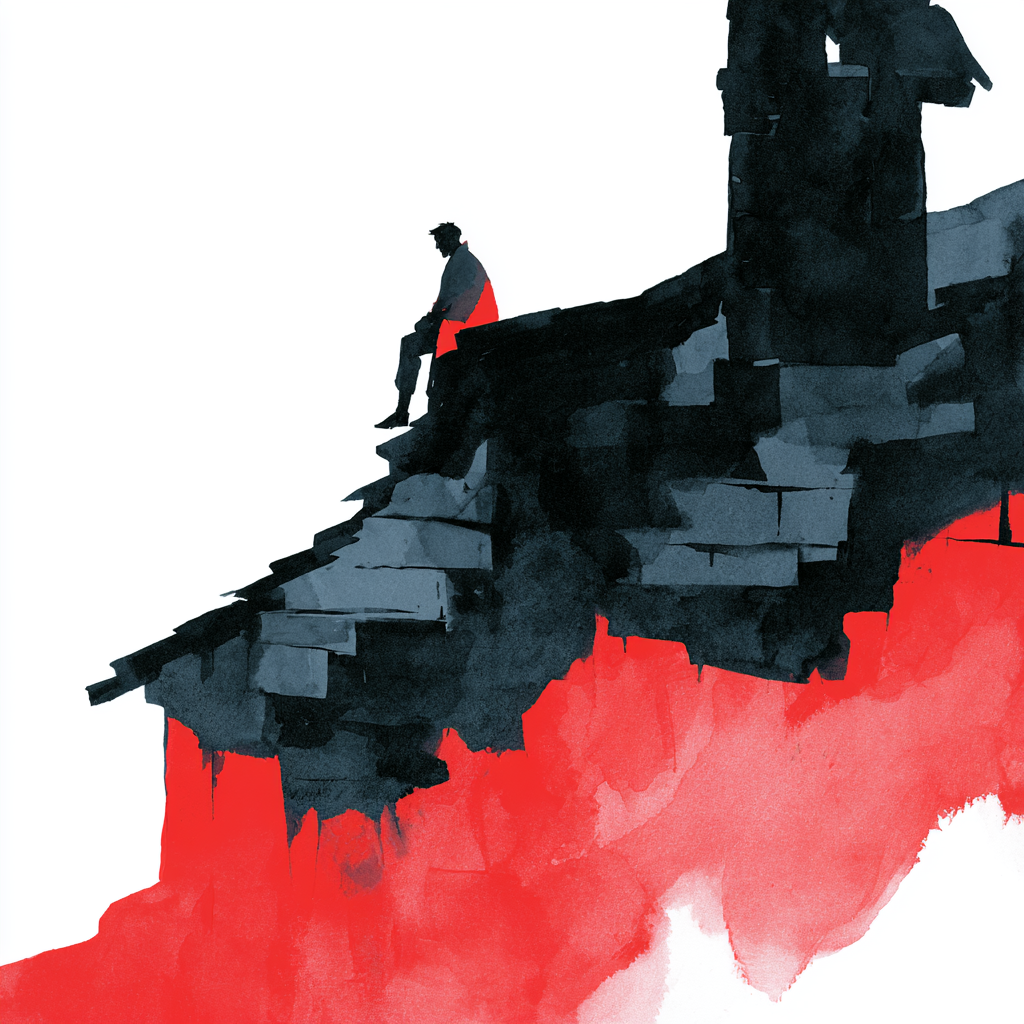
\includegraphics[keepaspectratio]{./images/man_in_the_roof.png}}

\chapter{Estratégia 29 -- Cobrir a árvore de
flores}\label{estratuxe9gia-29-cobrir-a-uxe1rvore-de-flores}

Melhorar a imagem de algo, para passar uma impressão diferente da real.
Popularmente, enfeitar a noiva para o casamento.

\pandocbounded{
\includegraphics[keepaspectratio]{./images/exhuberant_tree_with_lot_of_flowers.png}}

Um exemplo muito comum é o IPO (abertura de capital) de companhias em
bolsa de valores. Os executivos, muito interessados em fazer a abertura
de capital e embolsar uma pequena fortuna, fazem de tudo para que a
imagem e as contas da empresa pareçam boas, muitas vezes cortando gastos
de curto prazo e criando problemas de médio e longo prazo com isso.

\chapter{Estratégia 30 -- O convidado no papel do
anfitrião}\label{estratuxe9gia-30-o-convidado-no-papel-do-anfitriuxe3o}

Quando o anfitrião é fraco, e o convidado, forte, este assume o papel de
anfitrião e conduz a cerimônia.

\pandocbounded{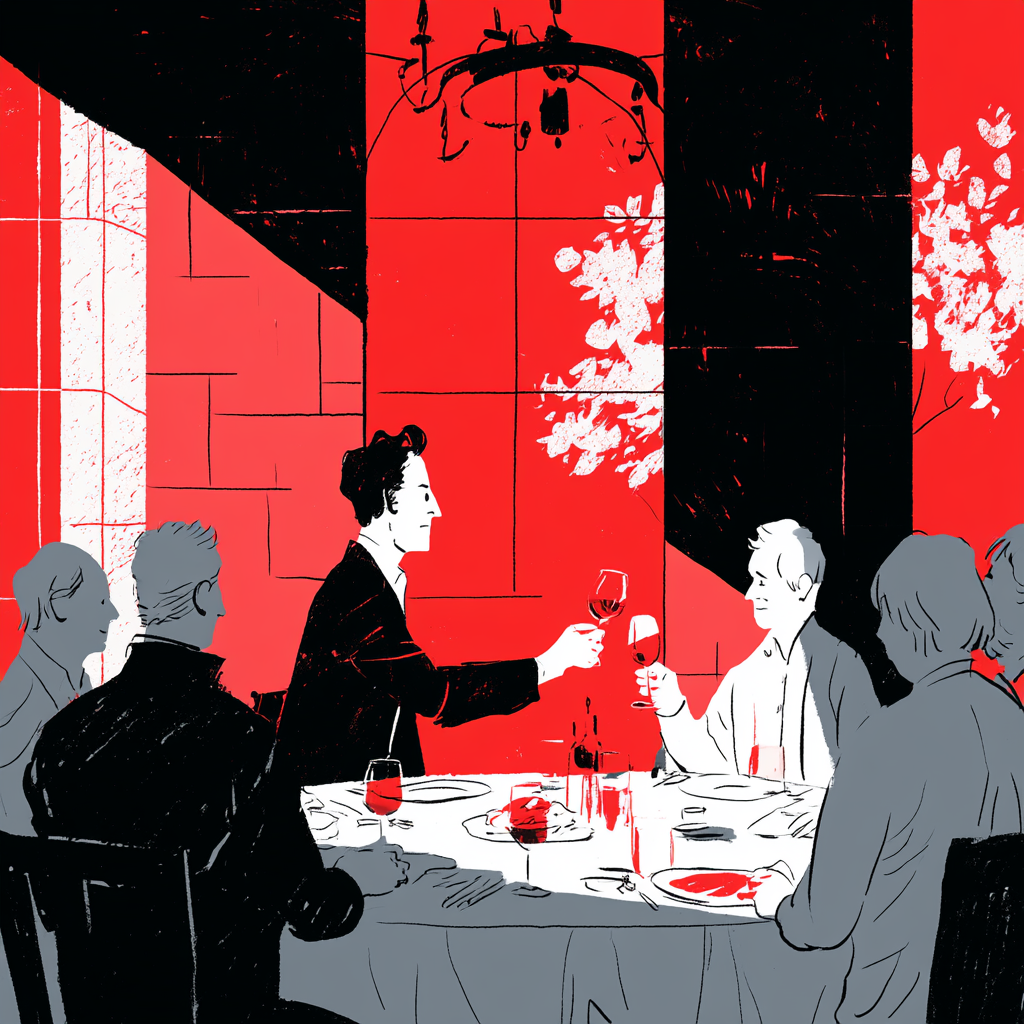
\includegraphics[keepaspectratio]{./images/toast.png}}

Exemplo. Entrevistas com políticos experientes. Independente da pergunta
que o jornalista faz, o político vai responder o que for melhor para
ele.

\part{31 a 36}

\chapter{Estratégias Desesperadas}\label{estratuxe9gias-desesperadas}

Compreendem as estratégias de 31 a 36.

\pandocbounded{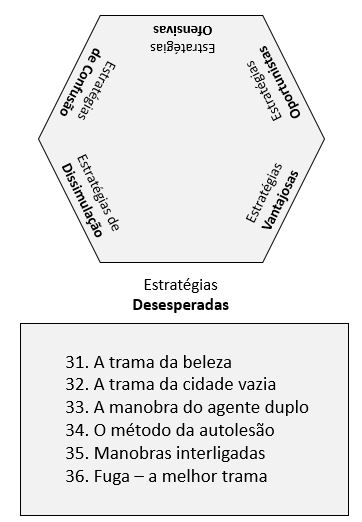
\includegraphics[keepaspectratio]{./images/36strategies_6.jpg}}

\href{estrategia_31.qmd}{31 -- A trama da beleza.}

\href{estrategia_32.qmd}{32 -- A trama da cidade vazia.}

\href{estrategia_33.qmd}{33 -- A manobra do agente duplo.}

\href{estrategia_34.qmd}{34 -- O método da autolesão.}

\href{estrategia_35.qmd}{35 -- Manobras interligadas.}

\href{estrategia_36.qmd}{36 -- Fuga -- a melhor trama.}

\chapter{Estratégia 31 -- A trama da
beleza}\label{estratuxe9gia-31-a-trama-da-beleza}

De forma geral, significa focar no ponto fraco do inimigo. Até mesmo os
mais poderosos generais (homens) são muito manipuláveis por mulheres
bonitas e charmosas.

Igualmente, as mulheres podem ser atraídas por belos varões.

A beleza encanta e é alvo de investigações filosóficas há tempos.

Um belo dashboard com um bom storytelling de dados pode persuadir os
diretores de uma empresa, mesmo que os dados em si estejam todos
errados.

Exemplos abundam na história. Sansão derrotado por Dalila, Betsabá
conquistando o coração de Davi -- e colocando o seu filho Salomão no
trono, Cleópatra, Helena de Troia, etc\ldots{}

``A mais antiga de todas as armas é a beleza. Aquilo que parece ser tão
belo pode ser tão letal'' - Zhao Er Hu

\chapter{Estratégia 32 -- A trama da cidade
vazia}\label{estratuxe9gia-32-a-trama-da-cidade-vazia}

É uma estratégia desesperada, para confundir o inimigo.

Vem de uma história ocorrida com o grande estrategista Zhuge Liang
KongMing. Ele estava encurralado pelo inimigo, e fez algo completamente
inesperado: simplesmente abriu os portões da cidade, e passou a varrer a
entrada, calmamente.

O oponente, que já tinha caído em várias armadilhas de KongMing,
desconfiou de alguma trama, e desistiu do ataque.

Para esta estratégia funcionar, deve-se ter bastante conhecimento
psicológico sobre o oponente.

\chapter{Estratégia 33 -- A manobra do agente
duplo}\label{estratuxe9gia-33-a-manobra-do-agente-duplo}

Utilizar o próprio espião do inimigo para disseminar informações falsas.

Sun Tzu dedica um capítulo inteiro da Arte da Guerra para o conceito de
espionagem. Aqui nas 36 estratégias, não é diferente, informação e
contra-informação são a forma de saber o que está acontecendo e planejar
ações.

\chapter{Estratégia 34 -- O método da
autolesão}\label{estratuxe9gia-34-o-muxe9todo-da-autolesuxe3o}

Causar dano a si mesmo, como forma de ganhar a confiança do inimigo.
Exemplo de um general chinês, que amputou o próprio braço para dizer que
tinha sido traído, mas na verdade era apenas um engodo para se infiltrar
entre os oficiais do inimigo.

Falsa modéstia é uma variação do método

\chapter{Estratégia 35 -- Manobras
interligadas}\label{estratuxe9gia-35-manobras-interligadas}

Utilização conjunta, serial ou paralela, das estratégias descritas
acima. Saber cada uma das estratégias é bom, mas saber qual utilizar,
quando, onde e como, é a verdadeira Arte da Guerra.

\pandocbounded{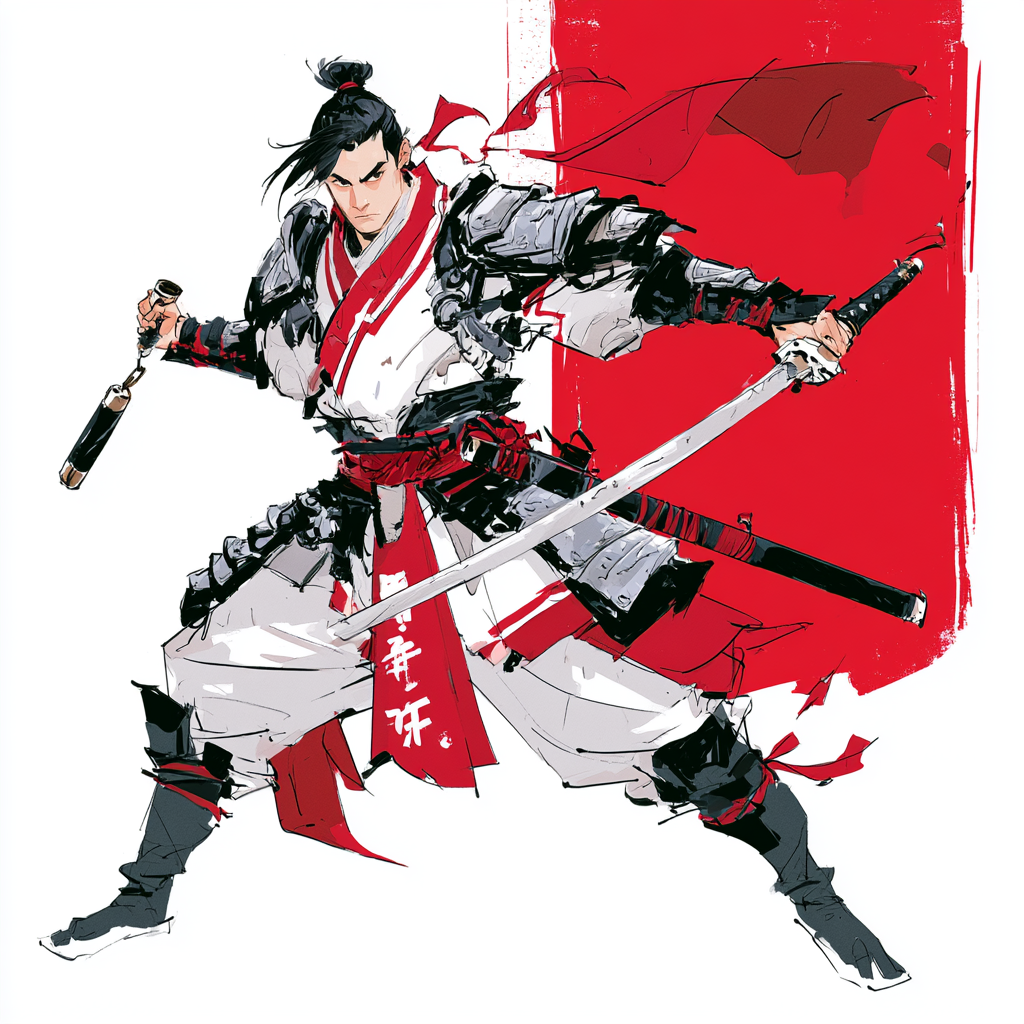
\includegraphics[keepaspectratio]{./images/warrior_nunchaku.png}}

\chapter{Estratégia 36 -- Fuga -- a melhor
trama}\label{estratuxe9gia-36-fuga-a-melhor-trama}

Se nada mais dar certo, fugir é uma excelente opção. Não há nada de
errado em se retrair hoje, para poder batalhar amanhã.

\pandocbounded{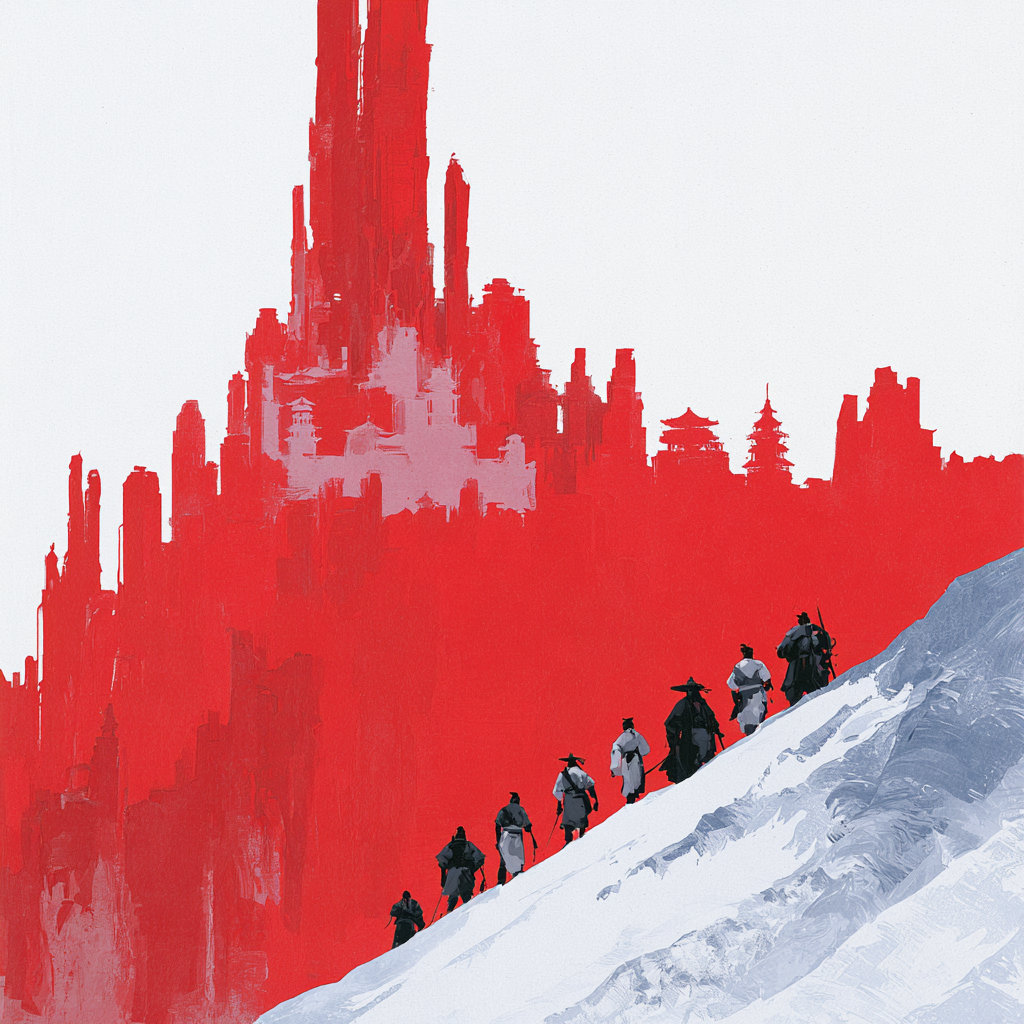
\includegraphics[keepaspectratio]{./images/running_away.png}}

\bookmarksetup{startatroot}

\chapter{Conclusão e Bibliografia
recomendada}\label{conclusuxe3o-e-bibliografia-recomendada}

Os 36 estratagemas é um dos tratados de guerra que são referência na
história da humanidade. Fiel ao estilo chinês, as estratégias são
descrições simples (originalmente escritas em 4 caracteres),
metafóricas, mas de significado profundo se compreendidas em sua
essência, e devastadoras quando aplicadas.

Há inumeráveis outros exemplos de uso, que abordo de quando em quando
neste espaço, e continuarei abordando, pelo tema ser muito rico, e pelo
ser humano ser extremamente complexo.

As 36 Estratégias dos Chineses por Wee Chow Hou
\pandocbounded{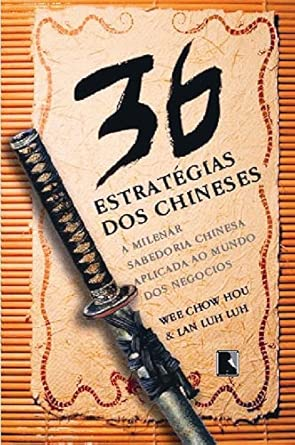
\includegraphics[keepaspectratio]{./images/36_estrategias.jpg}}

Lure the tiger out of the mountains: The thirty-six stratagems of
ancient China - Gao Yuan
\pandocbounded{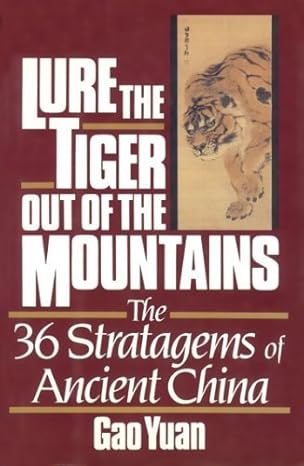
\includegraphics[keepaspectratio]{./images/Lure_tiger.jpg}}

A Arte Da Guerra - Sun Tzu
\pandocbounded{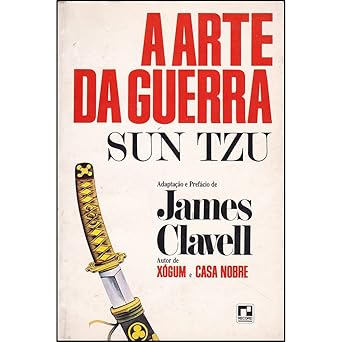
\includegraphics[keepaspectratio]{./images/arte_guerra.jpg}}

The 33 Strategies of War - Robert Greene
\pandocbounded{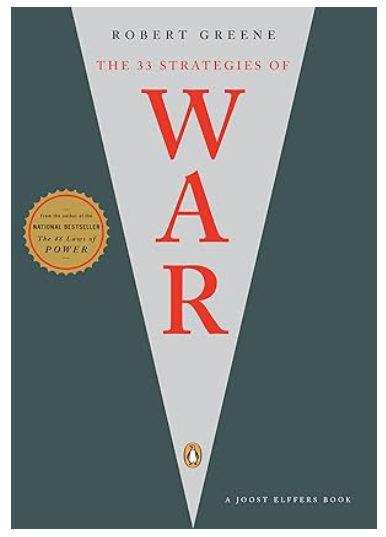
\includegraphics[keepaspectratio]{./images/33_strategies.png}}

\bookmarksetup{startatroot}

\chapter*{Sobre: Arnaldo Gunzi}\label{sobre-arnaldo-gunzi}
\addcontentsline{toc}{chapter}{Sobre: Arnaldo Gunzi}

\markboth{Sobre: Arnaldo Gunzi}{Sobre: Arnaldo Gunzi}

Sou apenas um curioso sobre a vida, a matemática aplicada e a
natureza\ldots{}

Minha missão: Traduzir Matemática Avançada + Dados + Conhecimento do
Negócio em valor real por meio de Analytics Avançado, IA e Otimização.

\pandocbounded{
\includegraphics[keepaspectratio]{images/arnaldo_gunzi_2026.jpeg}}

Tenho uma vasta experiência prática, em mais de 200 projetos, passando
por pela Stone, Mercado Livre, Klabin e Visagio.

Professor da XP Educação, Palestrante (de vez em quando alguém insano o
suficiente me convida para palestrar) e Escritor (blog, newsletter,
artigos).

Visite também:

\begin{itemize}
\item
  Meu LinkedIn: \url{https://www.linkedin.com/in/arnaldogunzi/}
\item
  O Compêndio de Ideias do Prof.~Arnaldo:
  \url{https://asgunzi.github.io/Compendium/}
\item
  Newsletter Reflexões Analíticas:
  \url{https://arnaldogunzi.substack.com/}
\item
  Blog pessoal: \url{https://ideiasesquecidas.com/}
\item
  Laboratório de Matemática: \url{https://asgunzi.neocities.org/}
\end{itemize}




\end{document}
